\title{Graph parsing by matrix multiplication}

\titlerunning{Graph parsing by matrix multiplication}

\author{Rustam Azimov}

\authorrunning{Rustam Azimov}

\tocauthor{Rustam Azimov}
\institute{St Petersburg State University\\
	\email{rustam.azimov19021995@gmail.com}}

\graphicspath{{Azimov/}}

\newtheorem{mytheorem}{Theorem}
\newtheorem{mydef}{Definition}
\renewcommand{\abstractname}{Abstract}
\renewcommand*{\proofname}{Proof}
\renewcommand*{\figurename}{Figure}
\renewcommand*{\tablename}{Table}
\renewcommand*{\refname}{References}

\maketitle

\begin{abstract}
Context-free path querying is a technique, which recently gains popularity in many areas, for example, graph databases, bioinformatics, static analysis, etc. The generalization of matrix-based Valiant's context-free language recognition algorithm for graph case is widely considered as a recipe for efficient context-free path querying; however, no progress has been made in this direction so far.
We propose the first generalization of matrix-based Valiant's algorithm for context-free and conjunctive path querying w.r.t relational and single-path query semantics. Our generalization does not deliver a truly sub-cubic worst-case complexity algorithm, whose existence still remains a hard open problem in the area. On the other hand, the utilization of matrix operations in the process of path query evaluation makes it possible to efficiently apply a wide class of optimizations and computing techniques, such as \textit{GPGPU}, parallel processing, sparse matrix representation, distributed-memory computation, etc.

\end{abstract}

\section*{Introduction}\label{sec:introduction}
In the era of big data and high load computations, graphical processing units
 (GPUs) are used extensively for data processing. 
 There have even been designed embedded devices with the support of GPUs
  for general purpose computations, like image recognition on mobile robots~\cite{NVJETSON}.
In practice many GPU-based applications tend to be bandwidth bound, meaning
 that data allocation and access are the main bottlenecks, thus memory optimizations
  appear to be in a prevailing significance and are addressed in a huge amount of research.

While the problem of available GPU memory could be tackled with sophisticated memory pooling techniques
 through memory swapping and sharing~\cite{zhang2019efficient},
  memory architecture of a GPU often requires more sophisticated optimizations.
   Given that a typical GPU incorporates several memory types, each having different
    capacity and throughput, a few memory management automation techniques have been introduced. They could leverage more effective memory spaces to handle register spilling and systematically consider the performance benefit achievable through a specific allocation of shared memory to save global memory transactions~\cite{AutomaticSharedMem,RegisterSpilling}. Further, the diversity of memory types imposes that each memory access should satisfy memory type specific patterns, to be most effective. Under the non-fulfillment of these patterns the data throughput of an application is aggravated due to the increase in the number of required memory transactions. Considering the following typical scenario of a GPU-accelerated application, another runtime memory optimization could be proposed.

 To facilitate the data processing a GPU routine is executed by multiple threads simultaneously with different pieces of data, often exceeding the maximal number of threads
  that could be executed simultaneously resulting in blocks of threads being executed iteratively.
 Being that the input data often exceeds the available GPU memory, the routine could not be applied at once, 
 and there is a need to split the data into chunks and process them iteratively 
 by the routine.
 It happens that some relatively small properties within a processing routine are maintained between the iterations
  and could be considered static in that sense.
 For example, if the application is a GPU-accelerated data processing engine that allows one to write queries to data and typically these queries remain small if compared to data and take significant execution time, the query, once specified by the user, can be used as a static, i.e. already known and constant, data for the query execution kernel runtime optimization since it remains unchanged during the host code execution.
 This observation allows to apply a \textit{partial evaluation} technique to optimize such routines in runtime.

\textit{Partial evaluation} or program \textit{specialization}~\cite{Jones1993,PartialEvalPaper} is a program
 transformation and optimization technique that optimizes a given program with
  respect to statically known inputs, producing another program which,
   if given only the remaining dynamic inputs, will produce the same results
    as initial one would have produced, given both inputs.
Basically, a partial evaluator performs an aggressive unfolding/unrolling, 
inlining, and constant propagation.  
The application of partial evaluation at runtime has 
recently shown a significant performance improvement of query execution for CPU-based
 database querying~\cite{LLVMmix}. 

Regarding memory optimizations of GPU kernels, partial evaluation is 
able to embed static data memory accesses into the code, i.e. place it directly 
into registers, once a kernel is properly written, which could result in a better
 performance compared to non-embedded access since memory transactions would be replaced 
 by accesses to the instruction cache. Thus, the aim of this work is to provide 
 an empirical evaluation of an existing partial evaluator AnyDSL~\cite{LeiBa} 
 that is capable of producing CUDA~\footnote{Programming and hardware model by NVIDIA.} code for NVIDIA GPUs
  to investigate the effects that appear after partially evaluating GPU applications,
   and what aspects of GPU architecture affect the desired result and 
   whether any significant performance improvements could be achieved at all.
   More specifically, the work performs the evaluation on string matching and convolutional filtering scenarios, providing some relevant CUDA assembly examples to ground the effects being observed.

\section{Background} \label{section_preliminaries}
In this section, we introduce the basic notions used throughout this work.

Let $\Sigma$ be a finite set of edge labels. Define an \textit{edge-labeled directed graph} as a tuple $D = (V, E)$ with a set of nodes $V$ and a directed edge-relation $E \subseteq V \times \Sigma \times V$.  For a path $\pi$ in a graph $D$, we denote the unique word obtained by concatenating the labels of the edges along the path $\pi$ as $l(\pi)$. Also, we write $n \pi m$ to indicate that a path $\pi$ starts at the node $n \in V$ and ends at the node $m \in V$.

Following Hellings~\cite{hellingsRelational}, we deviate from the usual definition of a context-free grammar in \textit{Chomsky Normal Form}~\cite{chomsky} by not including a special starting non-terminal, which will be specified in the path queries to the graph. Since every context-free grammar can be transformed into an equivalent one in Chomsky Normal Form and checking that an empty string is in the language is trivial it is sufficient to consider only grammars of the following type. A \textit{context-free grammar} is a triple $G = (N, \Sigma, P)$, where $N$ is a finite set of non-terminals, $\Sigma$ is a finite set of terminals, and $P$ is a finite set of productions of the following forms:

\begin{itemize}
    \item $A \rightarrow B C$, for $A,B,C \in N$,
    \item $A \rightarrow x$, for $A \in N$ and $x \in \Sigma$.   
\end{itemize}

Note that we omit the rules of the form $A \rightarrow \varepsilon$, where $\varepsilon$ denotes an empty string. This does not restrict the applicability of our algorithm because only the empty paths $m \pi m$ correspond to an empty string $\varepsilon$.

We use the conventional notation $A \xrightarrow{*} w$ to denote that a string $w \in \Sigma^*$ can be derived from a non-terminal $A$ by some sequence of applications of the production rules from $P$. The \textit{language} of a grammar $G = (N,\Sigma,P)$ with respect to a start non-terminal $S \in N$ is defined by $$L(G_S) = \{w \in \Sigma^*~|~S \xrightarrow{*} w\}.$$

For a given graph $D = (V, E)$ and a context-free grammar $G = (N, \Sigma, P)$, we define \textit{context-free relations} $R_A \subseteq V \times V$, for every $A \in N$, such that $$R_A = \{(n,m)~|~\exists n \pi m~(l(\pi) \in L(G_A))\}.$$

We define a binary operation $(~\cdot~)$ on arbitrary subsets $N_1 , N_2$ of $N$ with respect to a context-free grammar $G = (N, \Sigma, P)$ as $$N_1 \cdot N_2 = \{A~|~\exists B \in N_1, \exists C \in N_2 \text{ such that }(A \rightarrow B C) \in P\}.$$

Using this binary operation as a multiplication of subsets of $N$ and union of sets as an addition, we can define a \textit{matrix multiplication}, $a \times b = c$, where $a$ and $b$ are matrices of a suitable size that have subsets of $N$ as elements, as $$c_{i,j} = \bigcup^{n}_{k=1}{a_{i,k} \cdot b_{k,j}}.$$

According to Valiant~\cite{valiant}, we define the \textit{transitive closure} of a square matrix $a$ as $a^+ = a^{(1)}_+ \cup a^{(2)}_+ \cup \cdots$ where $a^{(1)}_+ = a$ and $$a^{(i)}_+ = \bigcup^{i-1}_{j=1}{a^{(j)}_+ \times a^{(i-j)}_+}, ~i \ge 2.$$

We enumerate the positions in the input string $s$ of Valiant's algorithm from 0 to the length of $s$. Valiant proposes the algorithm for computing this transitive closure only for upper triangular matrices, which is sufficient since for Valiant's algorithm the input is essentially a directed chain and for all possible paths $n \pi m$ in a directed chain $n < m$. In the context-free path querying input graphs can be arbitrary. For this reason, we need to compute the transitive closure of an arbitrary square matrix.

Also, the conjunctive grammars can be used in the path querying problems. Similar to the case of the context-free grammars, we deviate from the usual definition of a conjunctive grammar in the \textit{binary normal form}~\cite{okhotinConjAndBool} by not including a special start non-terminal, which will be specified in the queries to the graph. Since every conjunctive grammar can be transformed into an equivalent one in the binary normal form~\cite{okhotinConjAndBool} and checking that an empty string is in the language is trivial, then it is sufficient to only consider grammars of the following type. A \textit{conjunctive grammar} is 3-tuple $G = (N, \Sigma, P)$ where $N$ is a finite set of non-terminals, $\Sigma$ is a finite set of terminals, and $P$ is a finite set of productions of the following forms:

\begin{itemize}
	\item $A \rightarrow B_1 C_1~\& \ldots \&~B_m C_m$, for $m \geq 1$, $A,B_i,C_i \in N$,
	\item $A \rightarrow x$, for $A \in N$ and $x \in \Sigma$.   
\end{itemize}

For conjunctive grammars we also use the conventional notation $A \xrightarrow{*} w$ to denote that the string $w \in \Sigma^*$ can be derived from a non-terminal $A$ by some sequence of applying the production rules from $P$. The relation $\rightarrow$ is defined as follows:
\begin{itemize}
	\item Using a rule $A \rightarrow B_1 C_1~\& \ldots \&~B_m C_m \in P$, any atomic subterm $A$ of any term can be rewritten by the subterm $(B_1 C_1 ~\& \ldots \&~ B_m C_m)$:
	\begin{center}
		$\ldots A \ldots \rightarrow \ldots (B_1 C_1~\& \ldots \&~B_m C_m) \ldots$
	\end{center}
	\item A conjunction of several identical strings in $\Sigma^*$ can be rewritten by one such string: for every $w \in \Sigma^*$,
	\begin{center}
		$\ldots (w~\& \ldots \&~w) \ldots \rightarrow \ldots w \ldots$
	\end{center}
	
\end{itemize}

The \textit{language} of a conjunctive grammar $G = (N,\Sigma,P)$ with respect to a start non-terminal $S \in N$ is defined by $L(G_S) = \{w \in \Sigma^*~|~S \xrightarrow{*} w\}$.

For a given graph $D = (V, E)$ and a conjunctive grammar $G = (N, \Sigma, P)$, we define \textit{conjunctive relations} $R_A \subseteq V \times V$, for every $A \in N$, such that $R_A = \{(n,m)~|~\exists n \pi m~(l(\pi) \in L(G_A))\}$.

\section{Related works} \label{section_related}
Problems in many areas can be reduced to one of the formal-languages-constrained path problems~\cite{barrett2000formal}. For example, various problems of static code analysis~\cite{bastani2015specification,xu2009scaling} can be formulated in terms of the context-free language reachability~\cite{reps1998program} or in terms of the linear conjunctive language reachability~\cite{zhang2017context}. 

One of the well-known problems in the area of graph database analysis is the language-constrained path querying. For example, the regular language constrained path querying~\cite{reutter2017regular, fan2011adding, abiteboul1997regular, nole2016regular}, and the context-free language constrained path querying.

There are a number of solutions~\cite{hellingsRelational, GraphQueryWithEarley, RDF} for context-free path query evaluation w.r.t. the relational query semantics, which employ such parsing algorithms as CYK~\cite{kasami, younger} or Earley~\cite{Grune}. Other examples of path query semantics are single-path and \textit{all-path query semantics}. The all-path query semantics requires presenting all possible paths from node $m$ to node $n$ whose labeling is derived from a non-terminal $A$ for all triples $(A, m, n)$ evaluated using the relational query semantics. Hellings~\cite{hellingsPathQuerying} presented algorithms for the context-free path query evaluation using the single-path and the all-path query semantics. If a context-free path query w.r.t. the all-path query semantics is evaluated on cyclic graphs, then the query result can be an infinite set of paths. For this reason, in~\cite{hellingsPathQuerying}, annotated grammars are proposed as a possible solution.

In~\cite{GLL}, the algorithm for context-free path query evaluation w.r.t. the all-path query semantics is proposed. This algorithm is based on the generalized top-down parsing algorithm~---~GLL~\cite{scott2010gll}. This solution uses derivation trees for the result representation which is more native for grammar-based analysis. The algorithms in~\cite{GLL, hellingsPathQuerying} for the context-free path query evaluation w.r.t. the all-path query semantics can also be used for query evaluation using the relational and the single-path semantics.

Our work is inspired by Valiant~\cite{valiant}, who proposed an algorithm for general context-free recognition in less than cubic time. This algorithm computes the same parsing table as the CYK algorithm but does this by offloading the most intensive computations into calls to a Boolean matrix multiplication procedure. This approach not only provides an asymptotically more efficient algorithm but it also allows us to effectively apply GPGPU computing techniques. Valiant's algorithm computes the transitive closure $a^+$ of a square upper triangular matrix $a$. Valiant also showed that the matrix multiplication operation $(\times)$ is essentially the same as $|N|^2$ Boolean matrix multiplications, where $|N|$ is the number of non-terminals of the given context-free grammar in Chomsky normal form.

Hellings~\cite{hellingsRelational} presented an algorithm for the context-free path query evaluation using the relational query semantics. According to Hellings, for a given graph $D = (V, E)$ and a grammar $G = (N, \Sigma, P)$ the context-free path query evaluation w.r.t. the relational query semantics reduces to a calculation of the context-free relations $R_A$. Thus, in this work, we focus on the calculation of these context-free relations. Also, Hellings~\cite{hellingsRelational} presented an algorithm for the context-free path query evaluation using the single-path query semantics which evaluates paths of minimal length for all triples $(A,m,n)$, but also noted that the length of these paths is not necessarily upper bounded. Thus, in this work, we evaluate an arbitrary path for all triples $(A,m,n)$.

Yannakakis~\cite{transitive-closure} analyzed the reducibility of various path querying problems to the calculation of the transitive closure. He formulated a problem of Valiant's technique generalization to the context-free path query evaluation w.r.t. the relational query semantics. Also, he assumed that this technique cannot be generalized for arbitrary graphs, though it does for acyclic graphs.

Thus, the possibility of reducing the context-free path query evaluation using the relational and the single-path query semantics to the calculation of the transitive closure is an open problem.

Also, there is an algorithm~\cite{zhang2017context} for path querying with linear conjunctive grammars and relational query semantics. This grammars have no more than one nonterminal in each conjunct of the rule. Thus, the possibility of creating an algorithm for path query evaluation w.r.t. conjunctive grammars of an arbitrary form is an open problem.

\section{An algorithm for CFPQ using relational query semantics}
In this section, we show how the context-free path query evaluation using the relational query semantics can be reduced to the calculation of matrix transitive closure $a^{cf}$, prove the correctness of this reduction, introduce an algorithm for computing the transitive closure $a^{cf}$, and provide a step-by-step demonstration of this algorithm on a small example.

\subsection{Reducing CFPQ to transitive closure} \label{section_reducing}
In this section, we show how the context-free relations $R_A$ can be calculated by computing the matrix transitive closure $a^{cf}$.

We introduce another definition of the transitive closure of an arbitrary square matrix $a$ as $$a^{cf} = a^{(1)} \cup a^{(2)} \cup \cdots$$ where $a^{(1)} = a$ and $a^{(i)} = a^{(i-1)} \cup (a^{(i-1)} \times a^{(i-1)}), ~i \ge 2.$

To show that Valiant's and this definitions of the matrix transitive closure are equivalent, we introduce the partial order $\succeq$ on matrices with the fixed size which have subsets of $N$ as elements. For square matrices $a, b$ of the same size, we denote $a \succeq b$ iff $a_{i,j} \supseteq b_{i,j}$, for every $i, j$. For these two definitions of transitive closure, the following lemmas and theorem hold.

\begin{lemma}\label{lemma:cf_geq_valiant}
	Let $G =(N,\Sigma,P)$ be a grammar, let $a$ be a square matrix. Then $a^{(k)} \succeq a^{(k)}_+$ for any $k \geq 1$.
\end{lemma}
\begin{proof}(Proof by Induction)
	
	\textbf{Basis}: The statement of the lemma holds for $k = 1$, since $$a^{(1)} = a^{(1)}_+ = a.$$
	
	\textbf{Inductive step}: Assume that the statement of the lemma holds for any $k \leq (p - 1)$ and show that it also holds for $k = p$ where $p \geq 2$. For any $i \geq 2$ $$a^{(i)} = a^{(i-1)} \cup (a^{(i-1)} \times a^{(i-1)}) \Rightarrow a^{(i)} \succeq a^{(i-1)}.$$ Hence, by the inductive hypothesis, for any $i \leq (p-1)$ $$a^{(p-1)} \succeq a^{(i)} \succeq a^{(i)}_+.$$ Let $1 \leq j \leq (p - 1)$. The following holds $$(a^{(p-1)} \times a^{(p-1)}) \succeq (a^{(j)}_+ \times a^{(p-j)}_+),$$ since $a^{(p-1)} \succeq a^{(j)}_+$ and $a^{(p-1)} \succeq a^{(p-j)}_+$. By the definition, $$a^{(p)}_+ = \bigcup^{p-1}_{j=1}{a^{(j)}_+ \times a^{(p-j)}_+}$$ and from this it follows that $$(a^{(p-1)} \times a^{(p-1)}) \succeq a^{(p)}_+.$$ By the definition, $$a^{(p)} = a^{(p-1)} \cup (a^{(p-1)} \times a^{(p-1)}) \Rightarrow a^{(p)} \succeq (a^{(p-1)} \times a^{(p-1)}) \succeq a^{(p)}_+$$ and this completes the proof of the lemma.
\end{proof}

\begin{lemma}\label{lemma:valiant_geq_cf}
	Let $G =(N,\Sigma,P)$ be a grammar, let $a$ be a square matrix. Then for any $k \geq 1$ there is $j \geq 1$, such that $(\bigcup^{j}_{i=1}{a^{(i)}_+}) \succeq a^{(k)}$.
\end{lemma}
\begin{proof}(Proof by Induction)
	
	\textbf{Basis}: For $k = 1$ there is $j = 1$, such that $$a^{(1)}_+ = a^{(1)} = a.$$ Thus, the statement of the lemma holds for $k = 1$.
	
	\textbf{Inductive step}: Assume that the statement of the lemma holds for any $k \leq (p - 1)$ and show that it also holds for $k = p$ where $p \geq 2$. By the inductive hypothesis, there is $j \geq 1$, such that $$(\bigcup^{j}_{i=1}{a^{(i)}_+}) \succeq a^{(p-1)}.$$ By the definition, $$a^{(2j)}_+ = \bigcup^{2j-1}_{i=1}{a^{(i)}_+ \times a^{(2j-i)}_+}$$ and from this it follows that $$(\bigcup^{2j}_{i=1}{a^{(i)}_+}) \succeq (\bigcup^{j}_{i=1}{a^{(i)}_+}) \times (\bigcup^{j}_{i=1}{a^{(i)}_+}) \succeq (a^{(p-1)} \times a^{(p-1)}).$$ The following holds $$(\bigcup^{2j}_{i=1}{a^{(i)}_+}) \succeq a^{(p)} = a^{(p-1)} \cup (a^{(p-1)} \times a^{(p-1)}),$$ since $$(\bigcup^{2j}_{i=1}{a^{(i)}_+}) \succeq (\bigcup^{j}_{i=1}{a^{(i)}_+}) \succeq a^{(p-1)}$$ and $$(\bigcup^{2j}_{i=1}{a^{(i)}_+}) \succeq (a^{(p-1)} \times a^{(p-1)}).$$ Therefore there is $2j$, such that $$(\bigcup^{2j}_{i=1}{a^{(i)}_+}) \succeq a^{(p)}$$ and this completes the proof of the lemma.	
\end{proof}

\begin{mytheorem}\label{thm:closures}
	Let $G =(N,\Sigma,P)$ be a grammar, let $a$ be a square matrix. Then $a^+ = a^{cf}$.
\end{mytheorem}
\begin{proof}
	
	By the lemma~\ref{lemma:cf_geq_valiant}, for any $k \geq 1$, $a^{(k)} \succeq a^{(k)}_+$. Therefore $$a^{cf} = a^{(1)} \cup a^{(2)} \cup \cdots \succeq a^{(1)}_+ \cup a^{(2)}_+ \cup \cdots = a^+.$$ By the lemma~\ref{lemma:valiant_geq_cf}, for any $k \geq 1$ there is $j \geq 1$, such that $$(\bigcup^{j}_{i=1}{a^{(i)}_+}) \succeq a^{(k)}.$$ Hence $$a^+ = (\bigcup^{\infty}_{i=1}{a^{(i)}_+}) \succeq a^{(k)},$$ for any $k \geq 1$. Therefore $$a^+ \succeq a^{(1)} \cup a^{(2)} \cup \cdots = a^{cf}.$$ Since $a^{cf} \succeq a^+$ and $a^+ \succeq a^{cf}$, $$a^+ = a^{cf}$$ and this completes the proof of the theorem.
\end{proof}

Further, in this work, we use the transitive closure $a^{cf}$ instead of $a^+$ and, by the theorem~\ref{thm:closures}, an algorithm for computing $a^{cf}$ also computes Valiant's transitive closure $a^+$.

Let $G = (N,\Sigma,P)$ be a grammar and $D = (V, E)$ be a graph. We enumerate the nodes of the graph $D$ from 0 to $(|V| - 1)$. We initialize the elements of the $|V| \times |V|$ matrix $a$ with $\varnothing$. Further, for every $i$ and $j$ we set $$a_{i,j} = \{A_k~|~((i,x,j) \in E) \wedge ((A_k \rightarrow x) \in P)\}.$$ Finally, we compute the transitive closure $$a^{cf} = a^{(1)} \cup a^{(2)} \cup \cdots$$ where $$a^{(i)} = a^{(i-1)} \cup (a^{(i-1)} \times a^{(i-1)}),$$ for $i \ge 2$ and $a^{(1)} = a$. For the transitive closure $a^{cf}$, the following statements hold.

\begin{lemma}\label{lemma:cf}
Let $D = (V,E)$ be a graph, let $G =(N,\Sigma,P)$ be a grammar. Then for any $i, j$ and for any non-terminal $A \in N$, $A \in a^{(k)}_{i,j}$ iff $(i,j) \in R_A$ and $i \pi j$, such that there is a derivation tree of the height $h \leq k$ for the string $l(\pi)$ and a context-free grammar $G_A = (N,\Sigma,P,A)$.
\end{lemma}
\begin{proof}(Proof by Induction)

\textbf{Basis}: Show that the statement of the lemma holds for $k = 1$. For any $i, j$ and for any non-terminal $A \in N$, $A \in a^{(1)}_{i,j}$ iff there is $i \pi j$ that consists of a unique edge $e$ from the node $i$ to the node $j$ and $(A \rightarrow x) \in P$ where $x = l(\pi)$. Therefore $(i,j) \in R_A$ and there is a derivation tree of the height $h = 1$, shown in Figure~\ref{tree1}, for the string $x$ and a context-free grammar $G_A = (N,\Sigma,P,A)$. Thus, it has been shown that the statement of the lemma holds for $k = 1$.

\begin{figure}[h!]
 \centering
 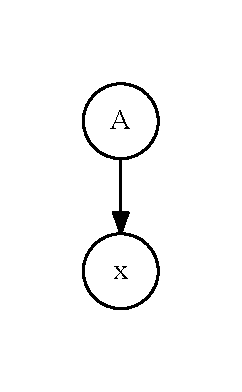
\includegraphics[width=0.2\textwidth]{pictures/tree1.pdf}
 \caption{The derivation tree of the height $h = 1$ for the string $x = l(\pi)$.}
 \label{tree1}
\end{figure}

\textbf{Inductive step}: Assume that the statement of the lemma holds for any $k \leq (p - 1)$ and show that it also holds for $k = p$ where $p \geq 2$. For any $i, j$ and for any non-terminal $A \in N$, $$A \in a^{(p)}_{i,j} \text{ iff } A \in a^{(p-1)}_{i,j} \text{ or } A \in (a^{(p-1)} \times a^{(p-1)})_{i,j},$$ since $$a^{(p)} = a^{(p-1)} \cup (a^{(p-1)} \times a^{(p-1)}).$$

Let $A \in a^{(p-1)}_{i,j}$. By the inductive hypothesis, $A \in a^{(p-1)}_{i,j}$ iff $(i,j) \in R_A$ and there exists $i \pi j$, such that there is a derivation tree of the height $h \leq (p-1)$ for the string $l(\pi)$ and a context-free grammar $G_A = (N,\Sigma,P,A)$. The statement of the lemma holds for $k = p$ since the height $h$ of this tree is also less than or equal to $p$.

Let $A \in (a^{(p-1)} \times a^{(p-1)})_{i,j}$. By the definition of the binary operation $(\cdot)$ on arbitrary subsets, $A \in (a^{(p-1)} \times a^{(p-1)})_{i,j}$ iff there are $r$, $B \in a^{(p-1)}_{i,r}$ and $C \in a^{(p-1)}_{r,j}$, such that $(A \rightarrow B C) \in P$. Hence, by the inductive hypothesis, there are $i \pi_1 r$ and $r \pi_2 j$, such that $(i,r) \in R_B$ and $(r,j) \in R_C$, and there are the derivation trees $T_B$ and $T_C$ of heights $h_1 \leq (p-1)$ and $h_2 \leq (p-1)$ for the strings $w_1 = l(\pi_1)$, $w_2 = l(\pi_2)$ and the context-free grammars $G_B$, $G_C$ respectively. Thus, the concatenation of paths $\pi_1$ and $\pi_2$ is $i \pi j$, where $(i,j) \in R_A$ and there is a derivation tree of the height $h = 1 + max(h_1, h_2)$, shown in Figure~\ref{tree2}, for the string $w = l(\pi)$ and a context-free grammar $G_A$.

\begin{figure}[h!]
 \centering
 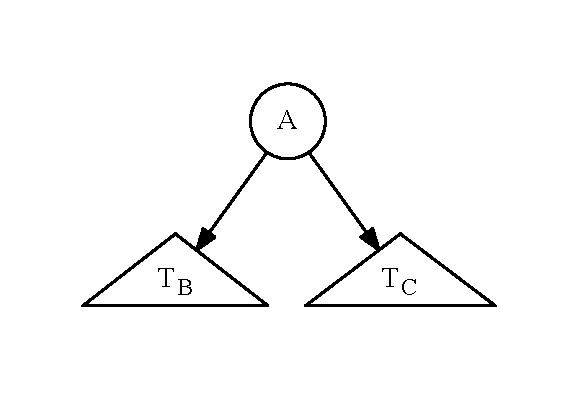
\includegraphics[width=0.8\textwidth]{pictures/tree2.pdf}
 \caption{The derivation tree of the height $h = 1 + max(h_1, h_2)$ for the string $w = l(\pi)$, where $T_B$ and $T_C$ are the derivation trees for strings $w_1$ and $w_2$ respectively.}
 \label{tree2}
\end{figure}

The statement of the lemma holds for $k = p$ since the height $h = 1 + max(h_1, h_2) \leq p$. This completes the proof of the lemma.
\end{proof}

\begin{mytheorem}\label{thm:correct}
 Let $D = (V,E)$ be a graph and let $G =(N,\Sigma,P)$ be a grammar. Then for any $i, j$ and for any non-terminal $A \in N$, $A \in a^{cf}_{i,j}$ iff $(i,j) \in R_A$.
\end{mytheorem}
\begin{proof}

Since the matrix $a^{cf} = a^{(1)} \cup a^{(2)} \cup \cdots,$ for any $i, j$ and for any non-terminal $A \in N$, $A \in a^{cf}_{i,j}$ iff there is $k \geq 1$, such that $A \in a^{(k)}_{i,j}$. By the lemma~\ref{lemma:cf}, $A \in a^{(k)}_{i,j}$ iff $(i,j) \in R_A$ and there is $i \pi j$, such that there is a derivation tree of the height $h \leq k$ for the string $l(\pi)$ and a context-free grammar $G_A = (N,\Sigma,P,A)$. This completes the proof of the theorem.
\end{proof}

We can, therefore, determine whether $(i,j) \in R_A$ by asking whether $A \in a^{cf}_{i,j}$. Thus, we show how the context-free relations $R_A$ can be calculated by computing the transitive closure $a^{cf}$ of the matrix $a$.



\subsection{The algorithm} \label{section_algorithm}
In this section, we introduce an algorithm for calculating the transitive closure $a^{cf}$ which was discussed in Section~\ref{section_reducing}.

Let $D = (V, E)$ be the input graph and $G = (N,\Sigma,P)$ be the input grammar.

\begin{algorithm}[H]
\begin{algorithmic}[1]
\caption{Context-free recognizer for graphs}
\label{alg:graphParse}
\Function{contextFreePathQuerying}{D, G}
    
    \State{$n \gets$ the number of nodes in $D$}
    \State{$E \gets$ the directed edge-relation from $D$}
    \State{$P \gets$ the set of production rules in $G$}
    \State{$T \gets$ the matrix $n \times n$ in which each element is $\varnothing$}
    \ForAll{$(i,x,j) \in E$}
    \Comment{Matrix initialization}
        \State{$T_{i,j} \gets T_{i,j} \cup \{A~|~(A \rightarrow x) \in P \}$}
    \EndFor    
    \While{matrix $T$ is changing}
       
        \State{$T \gets T \cup (T \times T)$}
        \Comment{Transitive closure $T^{cf}$ calculation} 
    \EndWhile
\State \Return $T$
\EndFunction
\end{algorithmic}
\end{algorithm}

Note that the matrix initialization in lines \textbf{6-7} of the Algorithm~\ref{alg:graphParse} can handle arbitrary graph $D$. For example, if a graph $D$ contains multiple edges $(i,x_1,j)$ and $(i,x_2,j)$ then both the elements of the set $\{A~|~(A \rightarrow x_1) \in P \}$ and the elements of the set $\{A~|~(A \rightarrow x_2) \in P \}$ will be added to $T_{i,j}$.

We need to show that the Algorithm~\ref{alg:graphParse} terminates in a finite number of steps. Since each element of the matrix $T$ contains no more than $|N|$ non-terminals, the total number of non-terminals in the matrix $T$ does not exceed $|V|^2|N|$. Therefore, the following theorem holds.

\begin{mytheorem}\label{thm:finite}
 Let $D = (V,E)$ be a graph and let $G =(N,\Sigma,P)$ be a grammar. The Algorithm~\ref{alg:graphParse} terminates in a finite number of steps. 
\end{mytheorem}
\begin{proof}
It is sufficient to show, that the operation in the line \textbf{9} of the Algorithm~\ref{alg:graphParse} changes the matrix $T$ only finite number of times. Since this operation can only add non-terminals to some elements of the matrix $T$, but not remove them, it can change the matrix $T$ no more than $|V|^2|N|$ times.
\end{proof}

Denote the number of elementary operations executed by the algorithm of multiplying two $n \times n$ Boolean matrices as $BMM(n)$. According to Valiant, the matrix multiplication operation in the line \textbf{9} of the Algorithm~\ref{alg:graphParse} can be calculated in $O(|N|^2 BMM(|V|))$. Denote the number of elementary operations executed by the matrix union operation of two $n \times n$ Boolean matrices as $BMU(n)$. Similarly, it can be shown that the matrix union operation in the line \textbf{9} of the Algorithm~\ref{alg:graphParse} can be calculated in $O(|N|^2 BMU(n))$. Since the line \textbf{9} of the Algorithm~\ref{alg:graphParse} is executed no more than $|V|^2|N|$ times, the following theorem holds.

\begin{mytheorem}\label{thm:time}
 Let $D = (V,E)$ be a graph and let $G =(N,\Sigma,P)$ be a grammar. The Algorithm~\ref{alg:graphParse} calculates the transitive closure $T^{cf}$ in $O(|V|^2|N|^3(BMM(|V|) + BMU(|V|)))$.
\end{mytheorem}

We also provide the worst-case example, for which the time complexity in terms of the graph size provided by Theorem~\ref{thm:time} cannot be improved. This example is based on the context-free grammar $G = (N, \Sigma, P)$ where:
\begin{itemize}
	\item the set of non-terminals $N = \{S\}$;
	\item the set of terminals $\Sigma = \{a, b\}$;
	\item the set of production rules $P$ is presented on Figure~\ref{ProductionRulesWorsCaseExample}.
\end{itemize}

\begin{figure}[h]
	\[
	\begin{array}{rccl}
	0: & S & \rightarrow & \text{\emph{a}} \ S \ \text{\emph{b}} \\
	1: & S & \rightarrow & \text{\emph{a}} \ \text{\emph{b}} \\ 
	\end{array}
	\]
	\caption{Production rules for the worst-case example.}
	\label{ProductionRulesWorsCaseExample}
\end{figure}

Let the size $|N|$ of the grammar $G$ be a constant. The worst-case time complexity is reached by running this query on the double-cyclic graph where:
\begin{itemize}
	\item one of the cycles having $u = 2^k + 1$ edges labeled with $a$;
	\item another cycle having $v = 2^k$ edges labeled with $b$;
	\item the two cycles are connected via a shared node $m$.
\end{itemize}

A small example of such graph with $k = 1$, $u = 3$, $v = 2$, and $m = 0$ is presented on Figure~\ref{worst_case_graph}.

\begin{figure}[h]
	\[
	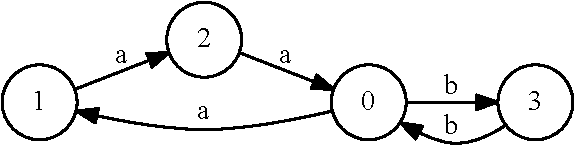
\includegraphics[width=0.8\textwidth]{pictures/worst_case_graph.pdf}
	\]
	\caption{An example of the graph for the worst-case time complexity.}
	\label{worst_case_graph}
\end{figure}

The shortest path $\pi$ from the node $m$ to the node $m$, whose labeling forms a string from the language $L(G_S)=\{a^n b^n; n \geq 1\}$, has a length $l = 2*u*v$, since $u = 2^k + 1$ and $v = 2^k$ are coprime, and string $s$, formed by this path, consists of $u*v$ labels $a$ and $u*v$ labels $b$. The string $s = l(\pi)$ has a derivation tree according to a context-free grammar $G_S$ of the minimal height $h = 2*u*v$ among all the paths from the node $m$ to the node $m$ in this double-cyclic graph. Therefore, if we run the worst-case example query on this graph, then the operation in the line \textbf{9} of the Algorithm~\ref{alg:graphParse} changes the matrix $T$ at least $h = 2*u*v$ times. Hence, the Algorithm~\ref{alg:graphParse} computes this query in $O(|V|^2(BMM(|V|) + BMU(|V|)))$, since $|V| = (u + v - 1) = 2*v$ and $h = 2*u*v > 2*v*v = |V|^2 / 4 = O(|V|^2)$.


\subsection{An example} \label{section_example}
In this section, we provide a step-by-step demonstration of the proposed algorithm. For this, we consider the classical \textit{same-generation query}~\cite{FndDB}.

The \textbf{example query} is based on the context-free grammar $G = (N, \Sigma, P)$ where:
\begin{itemize}
    \item The set of non-terminals $N = \{S\}$.
    \item The set of terminals $$\Sigma = \{subClassOf, subClassOf^{-1}, type, type^{-1}\}.$$
    \item The set of production rules $P$ is presented in Figure~\ref{ProductionRulesExampleQuery}.
\end{itemize}

\begin{figure}[h]
   \[
\begin{array}{rccl}
   0: & S & \rightarrow & \text{\textit{subClassOf}}^{-1} \ S \ \text{\textit{subClassOf}} \\ 
   1: & S & \rightarrow & \text{\textit{type}}^{-1} \ S \ \text{\textit{type}} \\ 
   2: & S & \rightarrow & \text{\textit{subClassOf}}^{-1} \ \text{\textit{subClassOf}} \\ 
   3: & S & \rightarrow & \text{\textit{type}}^{-1} \ \text{\textit{type}} \\ 
\end{array}
\]
\caption{Production rules for the example query grammar.}
\label{ProductionRulesExampleQuery}
\end{figure}

Since the proposed algorithm processes only grammars in Chomsky normal form, we first transform the grammar $G$ into an equivalent grammar $G' = (N', \Sigma', P')$ in normal form, where:
\begin{itemize}
    \item The set of non-terminals $N' = \{S, S_1, S_2, S_3, S_4, S_5, S_6\}$.
    \item The set of terminals $$\Sigma' = \{subClassOf, subClassOf^{-1}, type, type^{-1}\}.$$
    \item The set of production rules $P'$ is presented in Figure~\ref{ProductionRulesExampleQueryCNF}.
\end{itemize}

\begin{figure}[h]
   \[
\begin{array}{rccl}
   0: & S & \rightarrow & S_1 \ S_5 \\
   1: & S & \rightarrow & S_3 \ S_6 \\
   2: & S & \rightarrow & S_1 \ S_2 \\
   3: & S & \rightarrow & S_3 \ S_4 \\
   4: & S_5 & \rightarrow & S \ S_2 \\
   5: & S_6 & \rightarrow & S \ S_4 \\
   6: & S_1 & \rightarrow & \text{\textit{subClassOf}}^{-1} \\ 
   7: & S_2 & \rightarrow & \text{\textit{subClassOf}} \\ 
   8: & S_3 & \rightarrow & \text{\textit{type}}^{-1} \\
   9: & S_4 & \rightarrow & \text{\textit{type}} \\ 
\end{array}
\]
\caption{Production rules for the example query grammar in normal form.}
\label{ProductionRulesExampleQueryCNF}
\end{figure}

We run the query on a graph presented in Figure~\ref{ExampleQueryGraph}.

\begin{figure}[h]
\[
    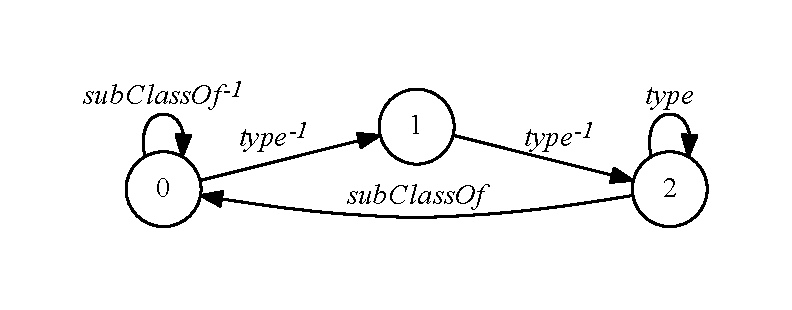
\includegraphics[width=0.8\textwidth]{pictures/ExampleGraph.pdf}
\]
\caption{An input graph for the example query.}
\label{ExampleQueryGraph}
\end{figure}

We provide a step-by-step demonstration of the work with the given graph $D$ and grammar $G'$ of the Algorithm~\ref{alg:graphParse}. After the matrix initialization in lines \textbf{6-7} of the Algorithm~\ref{alg:graphParse}, we have a matrix $T_0$ presented in Figure~\ref{ExampleQueryInitMatrix}.

\begin{figure}[h]
\[
T_0 = \begin{pmatrix}
    \{S_1\} & \{S_3\} & \varnothing \\ \varnothing & \varnothing & \{S_3\} \\ \{S_2\} & \varnothing & \{S_4\}
\end{pmatrix}
\]
\caption{The initial matrix for the example query.}
\label{ExampleQueryInitMatrix}
\end{figure}

Let $T_i$ be the matrix $T$ obtained after executing the loop in lines \textbf{8-9} of the Algorithm~\ref{alg:graphParse} $i$ times. The calculation of the matrix $T_1$ is shown in Figure~\ref{ExampleQueryFirstIteration}.

\begin{figure}[h]
\[
T_0 \times T_0 = \begin{pmatrix}
    \varnothing & \varnothing & \varnothing \\ \varnothing & \varnothing & \{S\} \\ \varnothing & \varnothing & \varnothing
\end{pmatrix}
\]

\[
T_1 = T_0 \cup (T_0 \times T_0) = \begin{pmatrix}
    \{S_1\} & \{S_3\} & \varnothing \\ \varnothing & \varnothing & \{S_3, S\} \\ \{S_2\} & \varnothing & \{S_4\}
\end{pmatrix}
\]
\caption{The first iteration of computing the transitive closure for the example query.}
\label{ExampleQueryFirstIteration}
\end{figure}

When the algorithm at some iteration finds new paths in the graph $D$, then it adds corresponding nonterminals to the matrix $T$. For example, after the first loop iteration, non-terminal $S$ is added to the matrix $T$. This non-terminal is added to the element with a row index $i = 1$ and a column index $j = 2$. This means that there is $i\pi j$ (a path $\pi$ from the node 1 to the node 2), such that $S \xrightarrow{*} l(\pi)$. For example, such a path consists of two edges with labels $type^{-1}$ and $type$, and thus $S \xrightarrow{*} type^{-1} \ type$.

The calculation of the transitive closure is completed after $k$ iterations when a fixpoint is reached: $T_{k-1} = T_k$. For the example query, $k = 6$ since $T_6 = T_5$. The remaining iterations of computing the transitive closure are presented in Figure~\ref{ExampleQueryFinalIterations}.

\begin{figure}[h]
\[
T_2 = \begin{pmatrix}
    \{S_1\} & \{S_3\} & \varnothing \\ \{S_5\} & \varnothing & \{S_3, S, S_6\} \\ \{S_2\} & \varnothing & \{S_4\}
\end{pmatrix}
\]

\[
T_3 = \begin{pmatrix}
    \{S_1\} & \{S_3\} & \{S\} \\ \{S_5\} & \varnothing & \{S_3, S, S_6\} \\ \{S_2\} & \varnothing & \{S_4\}
\end{pmatrix}
\]

\[
T_4 = \begin{pmatrix}
    \{S_1, S_5\} & \{S_3\} & \{S, S_6\} \\ \{S_5\} & \varnothing & \{S_3, S, S_6\} \\ \{S_2\} & \varnothing & \{S_4\}
\end{pmatrix}
\]

\[
T_5 = \begin{pmatrix}
    \{S_1, S_5, S\} & \{S_3\} & \{S, S_6\} \\ \{S_5\} & \varnothing & \{S_3, S, S_6\} \\ \{S_2\} & \varnothing & \{S_4\}
\end{pmatrix}
\]
\caption{Remaining states of the matrix $T$.}
\label{ExampleQueryFinalIterations}
\end{figure}

Thus, the result of the Algorithm~\ref{alg:graphParse} for the example query is the matrix $T_5 = T_6$. Now, after constructing the transitive closure, we can construct the context-free relations $R_A$. These relations for each non-terminal of the grammar $G'$ are presented in Figure~\ref{ExampleQueryCFRelations}.

\begin{figure}[h]
\begin{eqnarray*}
R_S&=&\{(0,0),(0,2),(1,2)\},\\
R_{S_1}&=&\{(0,0)\},\\
R_{S_2}&=&\{(2,0)\}, \\
R_{S_3}&=&\{(0,1), (1,2)\}, \\
R_{S_4}&=&\{(2,2)\}, \\
R_{S_5}&=&\{(0,0), (1,0)\}, \\
R_{S_6}&=&\{(0,2), (1,2)\}.
\end{eqnarray*}
\caption{Context-free relations for the example query.}
\label{ExampleQueryCFRelations}
\end{figure}

By the context-free relation $R_S$, we can conclude that there are paths in a graph $D$ only from the node 0 to the node 0, from the node 0 to the node 2 or from the node 1 to the node 2, corresponding to the context-free grammar $G_S$. This conclusion is based on the fact that a grammar $G'_S$ is equivalent to the grammar $G_S$ and $L(G_S) = L(G_S')$.

\section{CFPQ using single-path query semantics}
In this section, we show how the context-free path query evaluation using the single-path query semantics can be reduced to the calculation of matrix transitive closure $a^{cf}$ and prove the correctness of this reduction.

At the first step, we show how the calculation of matrix transitive closure $a^{cf}$ which was discussed in Section~\ref{section_reducing} can be modified to compute the length of some path $i \pi j$ for all $(i,j) \in R_A$, such that $A \xrightarrow{*} l(\pi)$. This is sufficient to solve the problem of context-free path query evaluation using the single-path query semantics since the required path of a fixed length from the node $i$ to the node $j$ can be found by a simple search and checking whether the labels of this path form a string which can be derived from a non-terminal $A$.

Let $G = (N,\Sigma,P)$ be a grammar and $D = (V, E)$ be a graph. We enumerate the nodes of the graph $D$ from 0 to $(|V| - 1)$. We initialize the $|V| \times |V|$ matrix $a$ with $\varnothing$. We associate each non-terminal in matrix $a$ with the corresponding path length. For convenience, each nonterminal $A$ in the $a_{i,j}$ is represented as a pair $(A,k)$ where $k$ is an associated path length. For every $i$ and $j$ we set $$a_{i,j} = \{(A_k,1)~|~((i,x,j) \in E) \wedge ((A_k \rightarrow x) \in P)\}$$ since initially all path lengths are equal to $1$. Finally, we compute the transitive closure $a^{cf}$ and if non-terminal $A$ is added to $a^{(p)}_{i,j}$ by using the production rule $(A \rightarrow B C) \in P$ where $(B,l_B) \in a^{(p-1)}_{i,k}$, $(C,l_C) \in a^{(p-1)}_{k,j}$, then the path length $l_A$ associated with non-terminal $A$ is calculated as $l_A = l_B + l_C$. Therefore $(A, l_A) \in a^{(p)}_{i,j}$. Note that if some non-terminal $A$ with an associated path length $l_1$ is in $a^{(p)}_{i,j}$, then the non-terminal $A$ is not added to the $a^{(k)}_{i,j}$ with an associated path length $l_2$ for all $l_2 \neq l_1$ and $k \geq p$. For the transitive closure $a^{cf}$, the following statements hold.

\begin{lemma}\label{lemma:singlepath}
	Let $D = (V,E)$ be a graph, let $G =(N,\Sigma,P)$ be a grammar. Then for any $i, j$ and for any non-terminal $A \in N$, if $(A,l_A) \in a^{(k)}_{i,j}$, then there is $i \pi j$, such that $A \xrightarrow{*} l(\pi)$ and the length of $\pi$ is equal to $l_A$.
\end{lemma}
\begin{proof}(Proof by Induction)
	
	\textbf{Basis}: Show that the statement of the lemma holds for $k = 1$. For any $i, j$ and for any non-terminal $A \in N$, $(A, l_A) \in a^{(1)}_{i,j}$ iff $l_A = 1$ and there is $i \pi j$ that consists of a unique edge $e$ from the node $i$ to the node $j$ and $(A \rightarrow x) \in P$ where $x = l(\pi)$. Therefore there is $i \pi j$, such that $A \xrightarrow{*} l(\pi)$ and the length of $\pi$ is equal to $l_A$. Thus, it has been shown that the statement of the lemma holds for $k = 1$.
	
	\textbf{Inductive step}: Assume that the statement of the lemma holds for any $k \leq (p - 1)$ and show that it also holds for $k = p$ where $p \geq 2$. For any $i, j$ and for any non-terminal $A \in N$, $(A, l_A) \in a^{(p)}_{i,j}$ iff $(A, l_A) \in a^{(p-1)}_{i,j}$ or $(A, l_A) \in (a^{(p-1)} \times a^{(p-1)})_{i,j}$ since $a^{(p)} = a^{(p-1)} \cup (a^{(p-1)} \times a^{(p-1)}).$
	
	Let $(A, l_A) \in a^{(p-1)}_{i,j}$. By the inductive hypothesis, there is $i \pi j$, such that $A \xrightarrow{*} l(\pi)$ and the length of $\pi$ is equal to $l_A$. Therefore the statement of the lemma holds for $k = p$.
	
	Let $(A, l_A) \in (a^{(p-1)} \times a^{(p-1)})_{i,j}$. By the definition, $(A, l_A) \in (a^{(p-1)} \times a^{(p-1)})_{i,j}$ iff there are $r$, $(B, l_B) \in a^{(p-1)}_{i,r}$ and $(C, l_C) \in a^{(p-1)}_{r,j}$, such that $(A \rightarrow B C) \in P$ and $l_A = l_B + l_C$. Hence, by the inductive hypothesis, there are $i \pi_1 r$ and $r \pi_2 j$, such that $$(B \xrightarrow{*} l(\pi_1)) \wedge(C \xrightarrow{*} l(\pi_2)),$$ where the length of $\pi_1$ is equal to $l_B$ and the length of $\pi_2$ is equal to $l_C$. Thus, the concatenation of paths $\pi_1$ and $\pi_2$ is $i \pi j$, where $A \xrightarrow{*} l(\pi)$ and the length of $\pi$ is equal to $l_A$. Therefore the statement of the lemma holds for $k = p$ and this completes the proof of the lemma.
\end{proof}

\begin{mytheorem}\label{thm:singlepathcorrect}
	Let $D = (V,E)$ be a graph and let $G =(N,\Sigma,P)$ be a grammar. Then for any $i, j$ and for any non-terminal $A \in N$, if $(A, l_A) \in a^{cf}_{i,j}$, then there is $i \pi j$, such that $A \xrightarrow{*} l(\pi)$ and the length of $\pi$ is equal to $l_A$.
\end{mytheorem}
\begin{proof}
	
	Since the matrix $a^{cf} = a^{(1)} \cup a^{(2)} \cup \cdots$, for any $i, j$ and for any non-terminal $A \in N$, if $(A, l_A) \in a^{cf}_{i,j}$, then there is $k \geq 1$, such that $A \in a^{(k)}_{i,j}$. By the lemma~\ref{lemma:singlepath}, if $(A, l_A) \in a^{(k)}_{i,j}$, then there is $i \pi j$, such that $A \xrightarrow{*} l(\pi)$ and the length of $\pi$ is equal to $l_A$. This completes the proof of the theorem.
\end{proof}

By the theorem~\ref{thm:correct}, we can determine whether $(i,j) \in R_A$ by asking whether $(A, l_A) \in a^{cf}_{i,j}$ for some $l_A$. By the theorem~\ref{thm:singlepathcorrect}, there is $i \pi j$, such that $A \xrightarrow{*} l(\pi)$ and the length of $\pi$ is equal to $l_A$. Therefore, we can find such a path $\pi$ of the length $l_A$ from the node $i$ to the node $j$ by a simple search. Thus, we show how the context-free path query evaluation using the single-path query semantics can be reduced to the calculation of matrix transitive closure $a^{cf}$. Note that the time complexity of the algorithm for context-free path querying w.r.t. the single-path semantics no longer depends on the Boolean matrix multiplications since we modify the matrix representation and operations on the matrix elements.

\section{A path querying algorithm using conjunctive grammars}
In this section, we show how the path querying using conjunctive grammars and relational query semantics can be reduced to the calculation of the matrix transitive closure. We propose an algorithm that calculates the over-approximation of all conjunctive relations $R_A$, since the query evaluation using the relational query semantics and conjunctive grammars is undecidable problem~\cite{hellingsRelational}.

We define a \textit{conjunctive matrix multiplication}, $a \circ b = c$, where $a$ and $b$ are matrices of the suitable size that have subsets of $N$ as elements, as $c_{i,j} = \{A~|~\exists (A \rightarrow B_1 C_1~\& \ldots \&~B_m C_m) \in P \text{ such that } (B_k, C_k) \in d_{i,j} \}$, where $d_{i,j} = \bigcup^{n}_{k=1}{a_{i,k} \times b_{k,j}}$ and $(\times)$ is the Cartesian product. 

We define the \textit{conjunctive transitive closure} of a square matrix $a$ as $a^{conj} = a^{(1)} \cup a^{(2)} \cup \cdots$ where $a^{(i)} = a^{(i-1)} \cup (a^{(i-1)} \circ a^{(i-1)})$, $i \ge 2$ and $a^{(1)} = a$.

\subsection{Reducing conjunctive path querying to transitive closure} \label{section_reducing_conj}
In this section, we show how the over-approximation of all conjunctive relations $R_A$ can be calculated by computing the transitive closure $a^{conj}$.

Let $G = (N,\Sigma,P)$ be a conjunctive grammar and $D = (V, E)$ be a graph. We number the nodes of the graph $D$ from 0 to $(|V| - 1)$ and we associate the nodes with their numbers. We initialize $|V| \times |V|$ matrix $b$ with $\emptyset$. Further, for every $i$ and $j$ we set $b_{i,j} = \{A_k~|~((i,x,j) \in E) \wedge ((A_k \rightarrow x) \in P)\}$. Finally, we compute the conjunctive transitive closure $b^{conj} = b^{(1)} \cup b^{(2)} \cup \cdots$ where $b^{(i)} = b^{(i-1)} \cup (b^{(i-1)} \circ b^{(i-1)})$, $i \ge 2$ and $b^{(1)} = b$. For the conjunctive transitive closure $b^{conj}$, the following statements holds.

\begin{lemma}\label{lemma:conj}
	Let $D = (V,E)$ be a graph, let $G =(N,\Sigma,P)$ be a conjunctive grammar. Then for any $i, j$ and for any non-terminal $A \in N$, if $(i,j) \in R_A$ and $i \pi j$, such that there is a derivation tree according to the string $l(\pi)$ and a conjunctive grammar $G_A = (N,\Sigma,P,A)$ of the height $h \leq k$ then $A \in b^{(k)}_{i,j}$.
\end{lemma}
\begin{proof}(Proof by Induction)
	
	\textbf{Basis}: Show that the statement of the lemma holds for $k = 1$. For any $i, j$ and for any non-terminal $A \in N$, if $(i,j) \in R_A$ and $i \pi j$, such that there is a derivation tree according to the string $l(\pi)$ and a conjunctive grammar $G_A = (N,\Sigma,P,A)$ of the height $h \leq 1$ then there is edge $e$ from node $i$ to node $j$ and $(A \rightarrow x) \in P$ where $x = l(\pi)$. Therefore $A \in b^{(1)}_{i,j}$ and it has been shown that the statement of the lemma holds for $k = 1$.
	
	\textbf{Inductive step}: Assume that the statement of the lemma holds for any $k \leq (p - 1)$ and show that it also holds for $k = p$ where $p \geq 2$. Let $(i,j) \in R_A$ and $i \pi j$, such that there is a derivation tree according to the string $l(\pi)$ and a conjunctive grammar $G_A = (N,\Sigma,P,A)$ of the height $h \leq p$.
	
	Let $h < p$. Then by the inductive hypothesis $A \in b^{(p-1)}_{i,j}$. Since $b^{(p)} = b^{(p-1)} \cup (b^{(p-1)} \circ b^{(p-1)})$ then $A \in b^{(p)}_{i,j}$ and the statement of the lemma holds for $k = p$.
	
	Let $h = p$. Let $A \rightarrow B_1 C_1~\& \ldots \&~B_m C_m$ be the rule corresponding to the root of the derivation tree from the assumption of the lemma. Therefore the heights of all subtrees corresponding to non-terminals $B_1, C_1, \ldots B_m, C_m$ are less than $p$. Then by the inductive hypothesis $B_x \in b^{(p-1)}_{i,t_x}$ and $C_x \in b^{(p-1)}_{t_x,j}$, for $x = 1\ldots m$ and $t_x \in V$. Let $d$ be a matrix that have subsets of $N \times N$ as elements, where $d_{i,j} = \bigcup^{n}_{t=1}{b^{(p-1)}_{i,t} \times b^{(p-1)}_{t,j}}$. Therefore $(B_x, C_x) \in d_{i,j}$, for $x = 1\ldots m$. Since $b^{(p)} = b^{(p-1)} \cup (b^{(p-1)} \circ b^{(p-1)})$ and $(b^{(p-1)} \circ b^{(p-1)})_{i,j} = \{A~|~\exists (A \rightarrow B_1 C_1~\& \ldots \&~B_m C_m) \in P \text{ such that } (B_k, C_k) \in d_{i,j} \}$ then $A \in b^{(p)}_{i,j}$ and the statement of the lemma holds for $k = p$. This completes the proof of the lemma.
\end{proof}

\begin{mytheorem}\label{thm:correct_conj}
	Let $D = (V,E)$ be a graph and let $G =(N,\Sigma,P)$ be a conjunctive grammar. Then for any $i, j$ and for any non-terminal $A \in N$, if $(i,j) \in R_A$ then $A \in b^{conj}_{i,j}$.
\end{mytheorem}
\begin{proof}
	
	By the lemma~\ref{lemma:conj}, if $(i,j) \in R_A$ then $A \in b^{(k)}_{i,j}$ for some $k$, such that $i \pi j$ with a derivation tree according to the string $l(\pi)$ and a conjunctive grammar $G_A = (N,\Sigma,P,A)$ of the height $h \leq k$. Since the matrix $b^{conj} = b^{(1)} \cup b^{(2)} \cup \cdots$, then for any $i, j$ and for any non-terminal $A \in N$, if $A \in b^{(k)}_{i,j}$ for some $k \geq 1$ then  $A \in b^{conj}_{i,j}$. Therefore, if $(i,j) \in R_A$ then $A \in b^{conj}_{i,j}$. This completes the proof of the theorem.
\end{proof}

Thus, we show how the over-approximation of all conjunctive relations $R_A$ can be calculated by computing the conjunctive transitive closure $b^{conj}$ of the matrix $b$.



\subsection{The algorithm} \label{section_algorithm_conj}
In this section we introduce an algorithm for calculating the conjunctive transitive closure $b^{conj}$ which was discussed in Section~\ref{section_reducing_conj}.

The following algorithm takes on input a graph $D = (V, E)$ and a conjunctive grammar $G = (N,\Sigma,P)$.

\begin{algorithm}[H]
	\begin{algorithmic}[1]
		\caption{Conjunctive recognizer for graphs}
		\label{alg:graphParse_conj}
		\Function{conjunctiveGraphParsing}{D, G}
		
		\State{$n \gets$ a number of nodes in $D$}
		\State{$E \gets$ the directed edge-relation from $D$}
		\State{$P \gets$ a set of production rules in $G$}
		\State{$T \gets$ a matrix $n \times n$ in which each element is $\emptyset$}
		\ForAll{$(i,x,j) \in E$}
		\Comment{Matrix initialization}
		\State{$T_{i,j} \gets T_{i,j} \cup \{A~|~(A \rightarrow x) \in P \}$}
		\EndFor    
		\While{matrix $T$ is changing}
		
		\State{$T \gets T \cup (T \circ T)$}
		\Comment{Transitive closure calculation} 
		\EndWhile
		\State \Return $T$    
		\EndFunction
	\end{algorithmic}
\end{algorithm}

Similar to the case of the context-free grammars we can show that the Algorithm~\ref{alg:graphParse_conj} terminates in a finite number of steps. Since each element of the matrix $T$ contains no more than $|N|$ non-terminals, then total number of non-terminals in the matrix $T$ does not exceed $|V|^2|N|$. Therefore, the following theorem holds.

\begin{mytheorem}\label{thm:finite_conj}
	Let $D = (V,E)$ be a graph and let $G =(N,\Sigma,P)$ be a conjunctive grammar. Algorithm~\ref{alg:graphParse_conj} terminates in a finite number of steps. 
\end{mytheorem}
\begin{proof}
	It is sufficient to show, that the operation in line \textbf{9} of the Algorithm~\ref{alg:graphParse_conj} changes the matrix $T$ only finite number of times. Since this operation can only add non-terminals to some elements of the matrix $T$, but not remove them, it can change the matrix $T$ no more than $|V|^2|N|$ times.
\end{proof}

\subsection{An example}
In this section, we provide a step-by-step demonstration of the proposed algorithm for path querying using conjunctive grammars. The \textbf{example query} is based on the conjunctive grammar $G = (N, \Sigma, P)$ in binary normal form where:
\begin{itemize}
	\item The set of non-terminals $N = \{S, A, B, C, D\}$.
	\item The set of terminals $\Sigma = \{a, b, c\}.$
	\item The set of production rules $P$ is presented in Figure~\ref{ProductionRulesExampleQueryConj}.
\end{itemize}

\begin{figure}[h]
	\[
	\begin{array}{rccl}
	0: & S & \rightarrow & AB \ \& \ DC \\ 
	1: & A & \rightarrow & a \\ 
	2: & B & \rightarrow & BC \\ 
	3: & B & \rightarrow & b \\
	4: & C & \rightarrow & c \\ 
	5: & D & \rightarrow & AD \\ 
	6: & D & \rightarrow & b \\ 
	\end{array}
	\]
	\caption{Production rules for the conjunctive example query grammar.}
	\label{ProductionRulesExampleQueryConj}
\end{figure}

The conjunct $AB$ generates the language $L_{AB} = \{abc^*\}$ and the conjunct $DC$ generates the language $L_{DC} = \{a^*bc\}$. Thus, the language generated by the conjunctive grammar $G_S = (N, \Sigma, P, S)$ is $L(G_S) = L_{AB} \cap L_{DC} = \{abc\}$. We tun the query on a graph presented in Figure~\ref{conjExampleGraph}.

\begin{figure}[h]
	\[
	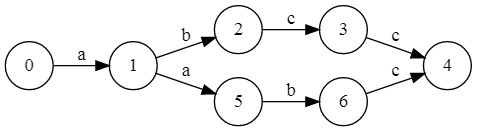
\includegraphics[width=0.8\textwidth]{pictures/ConjExampleGraph.png}
	\]
	\caption{An input graph for the conjunctive example query.}
	\label{conjExampleGraph}
\end{figure}

We provide a step-by-step demonstration of the work with the given graph $D$ and grammar $G$ of the Algorithm~\ref{alg:graphParse_conj}. After the matrix initialization in lines \textbf{6-7} of the Algorithm~\ref{alg:graphParse_conj}, we have a matrix $T_0$ presented in Figure~\ref{ConjExampleQueryInitMatrix}.

\begin{figure}[h]
	\[
	T_0 = \begin{pmatrix}
	\varnothing & \{A\} & \varnothing & \varnothing & \varnothing & \varnothing & \varnothing \\
	
	\varnothing & \varnothing & \{B, D\} & \varnothing & \varnothing & \{A\} & \varnothing \\
	
	\varnothing & \varnothing & \varnothing & \{C\} & \varnothing & \varnothing & \varnothing \\
	
	\varnothing & \varnothing & \varnothing & \varnothing & \{C\} & \varnothing & \varnothing \\
	
	\varnothing & \varnothing & \varnothing & \varnothing & \varnothing & \varnothing & \varnothing \\
	
	\varnothing & \varnothing & \varnothing & \varnothing & \varnothing & \varnothing & \{B, D\} \\
	
	\varnothing & \varnothing & \varnothing & \varnothing & \{C\} & \varnothing & \varnothing \\
	\end{pmatrix}
	\]
	\caption{The initial matrix for the example query.}
	\label{ConjExampleQueryInitMatrix}
\end{figure}

Let $T_i$ be the matrix $T$ obtained after executing the loop in lines \textbf{8-9} of the Algorithm~\ref{alg:graphParse_conj} $i$ times. To compute the matrix $T_1$ we need to compute the matrix $d$ where $d_{i,j} = \bigcup^{n}_{k=1}{T_{0_{i,k}} \times T_{0_{i,k}}}$. The matrix $d$ for the first loop iteration is presented in Figure~\ref{dmatrix}. The matrix $T_1 = $ $T_1 = T_0 \cup (T_0 \circ T_0)$ is shown in Figure~\ref{ConjExampleQueryFirstIteration}.

\begin{figure}[h]
	\noindent
	\resizebox{\linewidth}{!}{%
	$
	\begin{pmatrix}
	\varnothing & \varnothing & \{(A,B), (A,D)\} & \varnothing & \varnothing & \varnothing & \varnothing \\
	
	\varnothing & \varnothing & \varnothing & \{(B,C), (D,C)\} & \varnothing & \varnothing & \{(A,B), (A,D)\} \\
	
	\varnothing & \varnothing & \varnothing & \varnothing & \{(C,C)\} & \varnothing & \varnothing \\
	
	\varnothing & \varnothing & \varnothing & \varnothing & \varnothing & \varnothing & \varnothing \\
	
	\varnothing & \varnothing & \varnothing & \varnothing & \varnothing & \varnothing & \varnothing \\
	
	\varnothing & \varnothing & \varnothing & \varnothing & \{(B,C), (D,C)\} & \varnothing & \varnothing \\
	
	\varnothing & \varnothing & \varnothing & \varnothing & \varnothing & \varnothing & \varnothing \\
	\end{pmatrix}$%
	}
	\caption{The matrix $d$ for the first loop iteration.}
	\label{dmatrix}
\end{figure}

\begin{figure}[h]
	\[
	T_1 = \begin{pmatrix}
	\varnothing & \{A\} & \{D\} & \varnothing & \varnothing & \varnothing & \varnothing \\
	
	\varnothing & \varnothing & \{B, D\} & \{B\} & \varnothing & \{A\} & \{D\} \\
	
	\varnothing & \varnothing & \varnothing & \{C\} & \varnothing & \varnothing & \varnothing \\
	
	\varnothing & \varnothing & \varnothing & \varnothing & \{C\} & \varnothing & \varnothing \\
	
	\varnothing & \varnothing & \varnothing & \varnothing & \varnothing & \varnothing & \varnothing \\
	
	\varnothing & \varnothing & \varnothing & \varnothing & \{B\} & \varnothing & \{B, D\} \\
	
	\varnothing & \varnothing & \varnothing & \varnothing & \{C\} & \varnothing & \varnothing \\
	\end{pmatrix}
	\]
	\caption{The initial matrix for the example query.}
	\label{ConjExampleQueryFirstIteration}
\end{figure}

When the algorithm at some iteration finds new paths from the node $i$ to the node $j$ for all conjuncts of some production rule, then it adds nonterminal from the left side of this rule to the set $T_{i,j}$.

The calculation of the transitive closure is completed after $k$ iterations when a fixpoint is reached: $T_{k-1} = T_k$. For this example, $k = 4$ since $T_4 = T_3$. The remaining iterations of computing the transitive closure are presented in Figure~\ref{ConjExampleQueryFinalIterations}.

\begin{figure}
	\[
	T_2 = \begin{pmatrix}
	\varnothing & \{A\} & \{D\} & \{S\} & \varnothing & \varnothing & \{D\} \\
	
	\varnothing & \varnothing & \{B, D\} & \{B\} & \{S,B\} & \{A\} & \{D\} \\
	
	\varnothing & \varnothing & \varnothing & \{C\} & \varnothing & \varnothing & \varnothing \\
	
	\varnothing & \varnothing & \varnothing & \varnothing & \{C\} & \varnothing & \varnothing \\
	
	\varnothing & \varnothing & \varnothing & \varnothing & \varnothing & \varnothing & \varnothing \\
	
	\varnothing & \varnothing & \varnothing & \varnothing & \{B\} & \varnothing & \{B, D\} \\
	
	\varnothing & \varnothing & \varnothing & \varnothing & \{C\} & \varnothing & \varnothing \\
	\end{pmatrix}
	\]
	
	\[
	T_3 = \begin{pmatrix}
	\varnothing & \{A\} & \{D\} & \{S\} & \{S\} & \varnothing & \{D\} \\
	
	\varnothing & \varnothing & \{B, D\} & \{B\} & \{S,B\} & \{A\} & \{D\} \\
	
	\varnothing & \varnothing & \varnothing & \{C\} & \varnothing & \varnothing & \varnothing \\
	
	\varnothing & \varnothing & \varnothing & \varnothing & \{C\} & \varnothing & \varnothing \\
	
	\varnothing & \varnothing & \varnothing & \varnothing & \varnothing & \varnothing & \varnothing \\
	
	\varnothing & \varnothing & \varnothing & \varnothing & \{B\} & \varnothing & \{B, D\} \\
	
	\varnothing & \varnothing & \varnothing & \varnothing & \{C\} & \varnothing & \varnothing \\
	\end{pmatrix}
	\]
	
	\[
	T_4 = \begin{pmatrix}
	\varnothing & \{A\} & \{D\} & \{S\} & \{S\} & \varnothing & \{D\} \\
	
	\varnothing & \varnothing & \{B, D\} & \{B\} & \{S,B\} & \{A\} & \{D\} \\
	
	\varnothing & \varnothing & \varnothing & \{C\} & \varnothing & \varnothing & \varnothing \\
	
	\varnothing & \varnothing & \varnothing & \varnothing & \{C\} & \varnothing & \varnothing \\
	
	\varnothing & \varnothing & \varnothing & \varnothing & \varnothing & \varnothing & \varnothing \\
	
	\varnothing & \varnothing & \varnothing & \varnothing & \{B\} & \varnothing & \{B, D\} \\
	
	\varnothing & \varnothing & \varnothing & \varnothing & \{C\} & \varnothing & \varnothing \\
	\end{pmatrix}
	\]
	\caption{Remaining states of the matrix $T$.}
	\label{ConjExampleQueryFinalIterations}
\end{figure}

Thus, the result of the Algorithm~\ref{alg:graphParse_conj} for the example query is the matrix $T_4 = T_3$. Now, after constructing the transitive closure, we can construct the over-approximations $R'_A$ of the conjunctive relations $R_A$. These approximations for each non-terminal of the grammar $G$ are presented in Figure~\ref{ConjExampleQueryCFRelations}.

\begin{figure}
	\begin{eqnarray}
		R'_S&=&\{(0,3),(0,4),(1,4)\},\\
		R'_{A}&=&\{(0,1),(1,5)\},\\
		R'_{B}&=&\{(1,2),(1,3),(1,4),(5,4),(5,6)\}, \\
		R'_{C}&=&\{(2,3),(3,4),(6,4)\}, \\
		R'_{D}&=&\{(0,2),(0,6),(1,2),(1,6),(5,6)\}.
	\end{eqnarray}
	\caption{The over-approximations of the conjunctive relations for the example query.}
	\label{ConjExampleQueryCFRelations}
\end{figure}

This example demonstrates that it is not always possible to obtain an exact solution. For example, a pair of nodes $(0,4)$ belongs to $R'_S$, although there is no path from the node $0$ to the node $4$, which forms a string derived from the nonterminal $S$ (only the string $abc$ can be derived from the nonterminal $S$). Extra pairs of nodes are added if there are different paths from the node $i$ to the node $j$, which in summary correspond to all conjuncts of one production rule, but there is no path from the node $i$ to the node $j$, which at the same time would correspond to all conjuncts of this rule. For example, for the conjuncts of the rule $S \rightarrow AB \ \& \ DC$, there is a path from the node $0$ to the node $4$ forming the string $abcc$, and there is also a path from the node $0$ to the node $4$ forming the string $aabc$. The first path corresponds to the conjunct $AB$, since the string $abcc$ belongs to the language $L_{AB} = \{abc^*\}$, and the second path corresponds to the conjunct $DC$, since the string $aabc$ belongs to the language $L_{DC} = \{a^*bc\}$. However, it is obvious that there is no path from the node $0$ to the node $4$, which forms the string $abc$.

\section{Evaluation}
In this section, the implementation details of the benchmarks are provided, 
as well as the selected datasets, and GPU architecture details that affect 
the result. A general workflow of analyzing GPU-code is also could be seen 
in this section. 

\subsection{String matching}
GPU-accelerated string matching frequently appears in GPU-based data\-bases, 
file carving~\cite{DataCarving,GPU-carving} that stands for extracting 
files from raw data in a field of cyber forensics, and intrusion 
detection~\cite{GPU-IDS}. Thus such a problem has a huge practical 
interest. Substrings could be considered static and subjected to 
partial evaluation.

\subsubsection{Na\`ive single substring matching}\label{naive-single}
Na\`ive algorithm operates on a \emph{subject} string and a \emph{pattern}, 
iteratively comparing each symbol of the pattern with the 
symbols of each substring of the subject string of size equal to the size 
of the pattern. The algorithm is inherently data-parallel: such substrings 
could be traversed separately, each in their thread. Further, such a traversal 
provides a rather optimal global memory access pattern, since adjacent 
threads would access addresses of adjacent substrings. There exist an opportunity 
for optimization, since at one moment all threads in a warp access the same symbol 
of the pattern (and distinct symbols of the subject string), thus the pattern could 
be placed in constant memory to speed up the performance.

%<3 pushishku <3
 
There is a \emph{KMP} test for optimizers like partial evaluator, 
intended to check whether they correctly reduce static computations. 
Partial evaluation is able to reduce a na\`ive single substring matching, 
though properly rewritten, to something very like Knuth--Morris--Pratt algorithm~\cite{KMP-Danvy}, 
which uses a prefix function to recover from a mismatch, thus being linear with 
respect to the subject string.
When a mismatch occurs, it is known that all previous symbols of the pattern 
match the ones of the substring of the subject string up to the point of mismatch. 
In order to simulate a prefix function at the mismatch point, the pattern could be 
matched against itself up to this point, searching for the largest prefix being a 
suffix as well.
Since the pattern is static and matched against itself, this computation is fully static 
and could be performed at specialization time.
Porting this approach to GPU and Impala, and applying partial evaluation 
at runtime indeed produces a KMP-like program\footnote{\url{https://github.com/Tiltedprogrammer/spec/blob/master/kmp.dump}\\ (last accessed date: 30.05.2020)}. 
Thus, making the used partial evaluator sound in a sense. The KMP algorithm itself is hard to partially evaluate since the already matched piece of the pattern 
that drives the search through the backtracking table is fully dynamic.

However, such an approach is far less data parallel as well as KMP. The subject 
string should be divided into interleaved chunks, each assigned to a different 
thread. Such parallelization has a far worse access pattern since each 
thread accesses strided addresses of the subject string. 
However, in practice, such an access pattern occurs when the search is performed 
across different subject strings, where each thread operates on a 
specific string\footnote{\url{https://github.com/NVIDIA/nvstrings} \\(last accessed date: 30.05.2020)}

A na\`ive single substring matching could be also specialized by simply unrolling 
the traversal, that does not hurt the parallelization. 
The evaluation of these approaches is presented in figure~\ref{fig:kmp_test}.

\begin{figure}
    \centering
    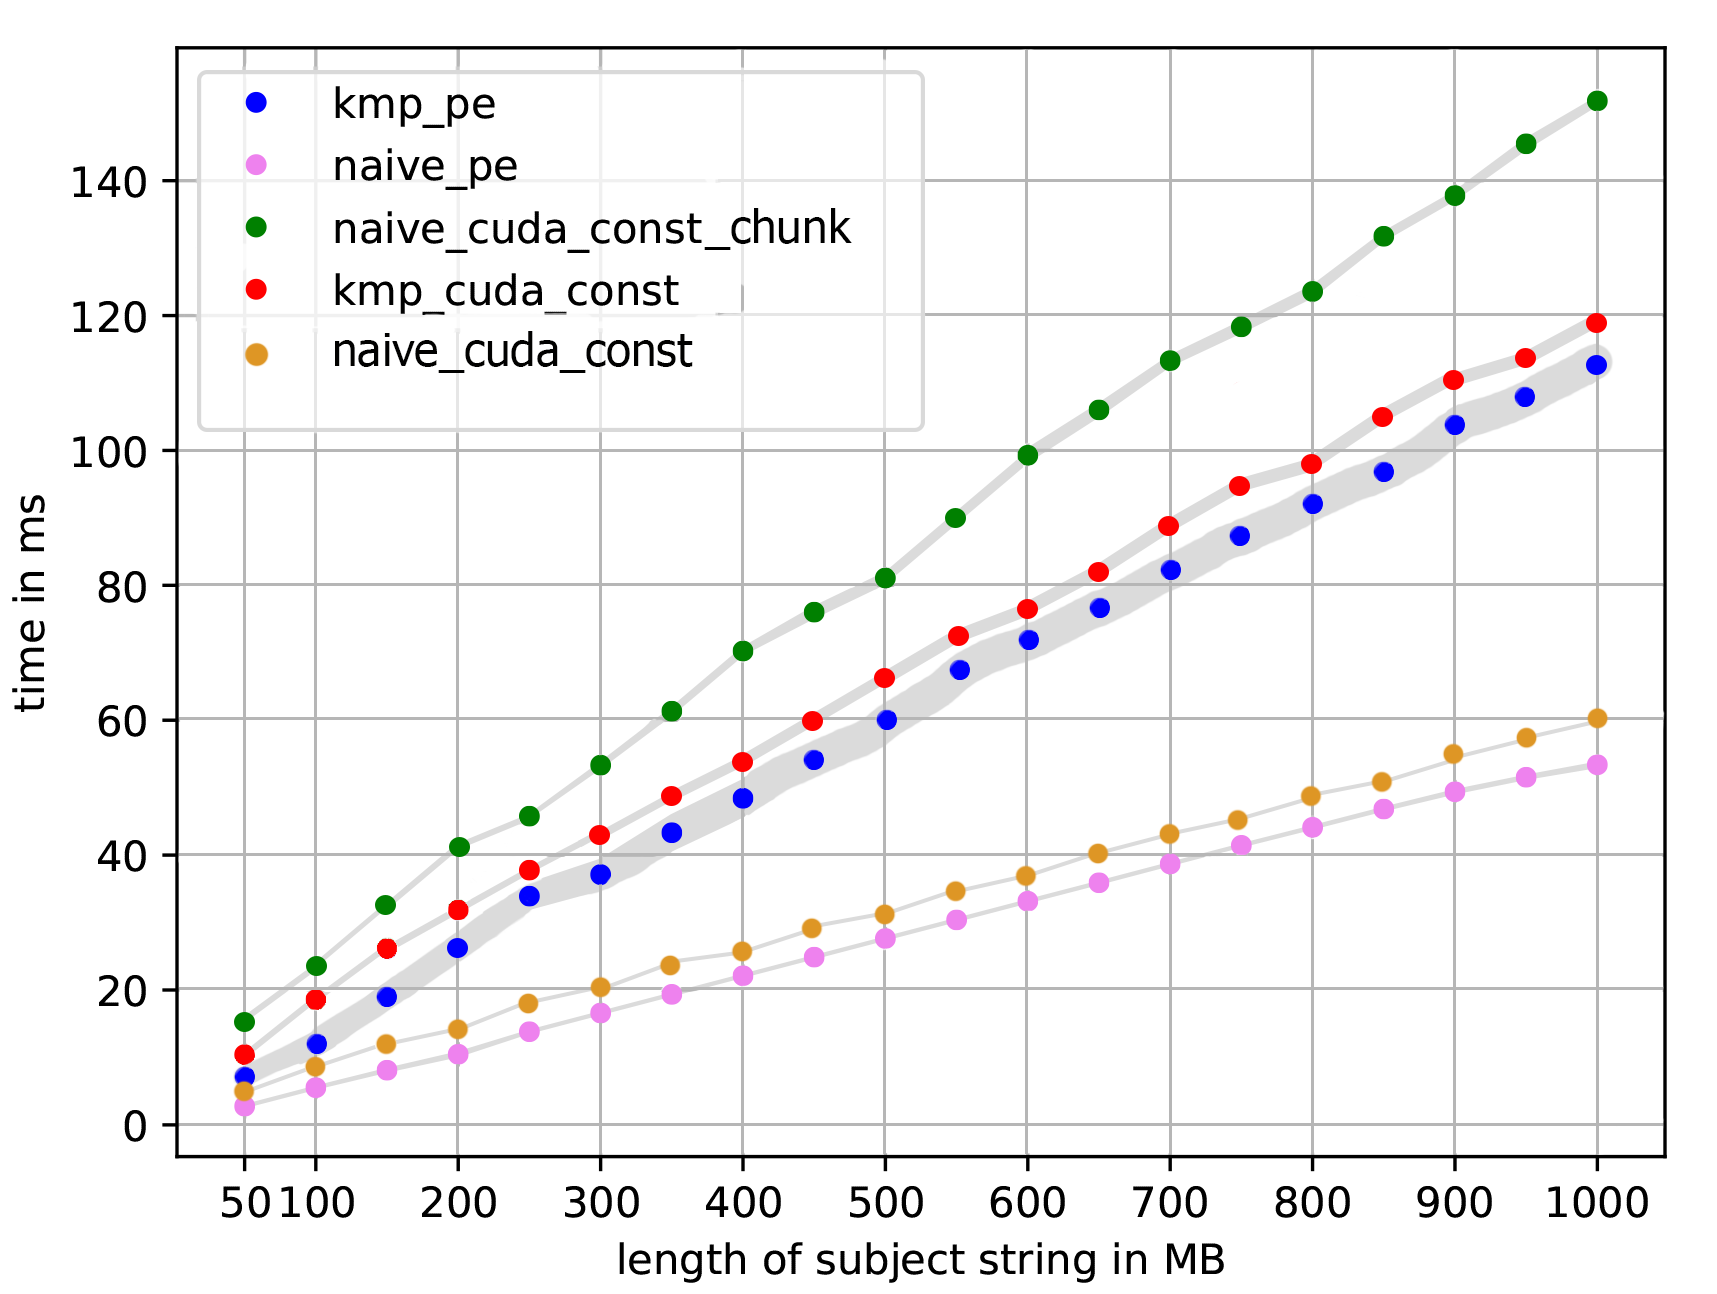
\includegraphics[width=0.85\linewidth]{figures/KMP_TEST.png}
    \caption{Na\`ive single substring matching}
    \label{fig:kmp_test}
\end{figure}

The current recursive implementation of the partial evaluator does not 
handle well the KMP test with patterns of more than 16 bytes in length. 
Thus, for the evaluation, a set of uniformly randomized 50 patterns\footnote{Enough for the divergence not to affect deviation so much.} 
from two-characters alphabet has been taken, satisfying that restriction. The subject string has been also randomly generated from the same alphabet. The standard deviation is shown in gray regions.
The KMP algorithm obtained by partial evaluation (\emph{kmp\_pe}), KMP algorithm implemented with CUDA, utilizing constant memory to store the backtrack table and the pattern (\emph{kmp\_cuda\_const}), 
na\`ive algorithm in CUDA with chunk-based parallelization (\emph{naive\_cuda\_const}), naive\`ive algorithm in CUDA with char-based parallelization and its partially evaluated version, that embeds the 
pattern into the code through unrolling the traversal, are compared. The figure grounds the success of the KMP test and shows that data embedding does not give any significant improvements: the difference 
between embedded and not embedded versions are mainly due to the reduced amount of address computations and loop overhead. The char-based parallel version is at the bottom due to a better memory access policy.

\subsubsection{Data embedding}\label{data_embedding}
Partial evaluation for the scenario above performed the transformation 
similar to the one in listing~\ref{code:kmp_spec}. While the load/store 
speed comparison for memory spaces is well described~\cite{TeslaT4Bench}, 
e.g. non-conflicting constant load is faster than L1 cache hit, the behavior 
of such embedded data is unspecified, but could be deduced as follows.
Embedded values could either inhabit a register, when e.g. \mintinline{C}{MOV R1 0x62}
 instruction occurs or be immediate-value parameters of the instructions. 
  The mini benchmark from listing~\ref{code:mem_bench} shows that embedded values are accessed through instruction cache by measuring the
   number of cycles required to perform an addition operation
   \mintinline{LLVM}{add.u32} with one of the arguments passed via embedded value or 
   via constant memory, lines 9 and 13. Given such a benchmark, the version with the value 
   embedded performs 10 times faster: 42 cycles versus 430 on a constant cache miss. If the constant 
   cache is firstly warmed up, the latency becomes 42 cycles and is the same for both instructions. 
   Thus, embedded values are more likely to be accessed via instruction memory, since 
   the instructions are prefetched and would outperform constant memory access under cache misses. 
   
   \begin{listing}
    \begin{pyglist}[language=C, caption=Memory benchmark,label=code:mem_bench]
__constant__ int mini_array [2];
    
__global__ void dummy_kernel(int* dst,int* clocks){
        
    int i;
    int start,stop;
        
    asm volatile("mov.u32 %0, %%clock;": "=r"(start) :: "memory");
    asm volatile(
                "add.u32 %0, %1, 12;\n\t"
                :"=r"(i) :"r"(i): "memory");
    // vs
    asm volatile(
                "add.u32 %0, %1,%2;\n\t"
                :"=r"(i) :"r"(i),"r"(mini_array[0]: "memory");
    asm volatile("mov.u32 %0, %%clock;": "=r"(stop) :: "memory");
    }
    \end{pyglist}
    \end{listing}

   Notably, when embedding, a partial evaluator is able to generate a more effective instruction, e.g. 
   shift instead of division, which takes more than 10 instructions on GPU, 
   while shift requires only one.

\begin{listing}
\begin{pyglist}[language=C,caption=KMP partial evaluation,label=code:kmp_spec]
    //kmp_cuda_const
LDC R0, c[0x3][R0] //load pattern's character
    //...//
    
LDG R12, [R2] //load subject's character
ISETP.NE.AND P0, R0, R12 // compares
    //..//

LDC R4, c[0x3][R2] // in case of mismatch go to backtrack position

    //kmp_pe
LDG R12, [R2] //load subject's character from global memory
    //    ...
ISETP.NE.AND P0, R12, 0x61 // pattern's char is put into the instruction
\end{pyglist}
\end{listing}

\subsubsection{Na\`ive multiple substring matching}\label{nmsm}

\begin{figure}
    \centering
    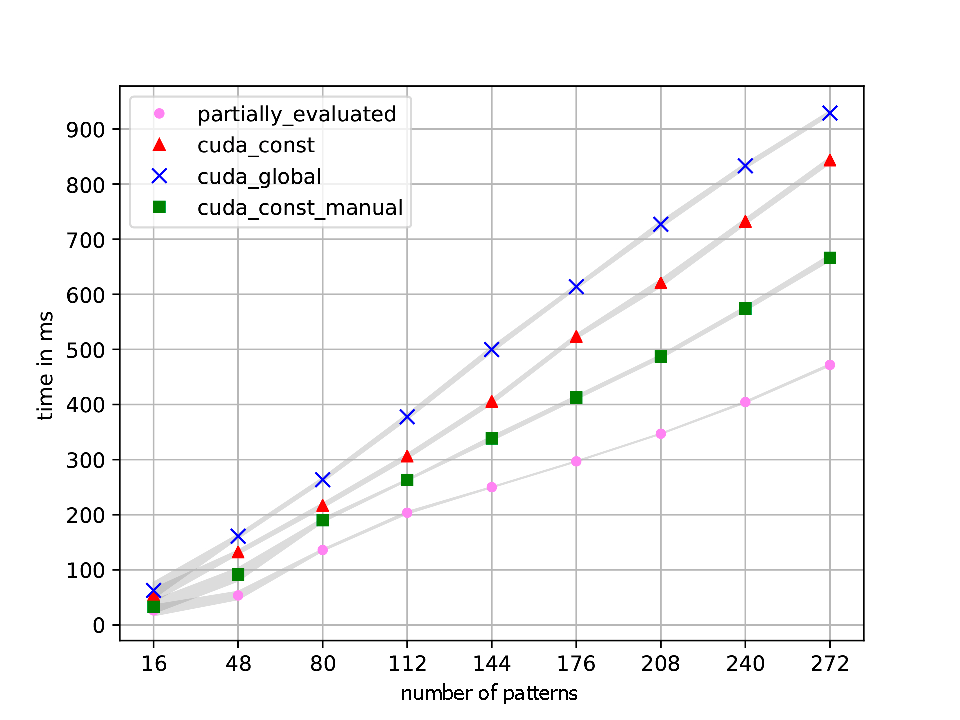
\includegraphics[width=0.85\linewidth]{figures/PredDefendNaiveSearch.pdf}
    \caption{Na\`ive multiple substring matching}
    \label{fig:naive_multy}
\end{figure}

The core of the algorithm is the same as the one of~\ref{naive-single} with the addition that a set of patterns is traversed against the substring. Since a set of patterns is traversed, their sizes are needed to be accessed, in order to be able to determine the border between the patterns. Constant memory could be utilized to store the sizes and the patterns, since threads of a warp access the same size and the same symbol of the pattern. Partially evaluating the algorithm with respect to the patterns, allows to fully reduce all the memory accesses to the sizes, which are numerous when the subject string is huge. Partial evaluation is achieved through loop unrolling for the sizes and the patterns. The results of this benchmark are presented in figure~\ref{fig:naive_multy}.

The dataset under use is from the intrusion detection area, which is common for multiple pattern matching problems~\cite{Aho-Corasick}. 
The subject string is 500MB \emph{tcpdump} from \emph{Botnet} 
dataset~\cite{Ring_2019}. The patterns are extracted from 
\emph{Snort V3}\footnote{\url{https://www.snort.org/downloads} (last accessed date: 30.05.2020)} 
rules, which are the patterns containing malicious traffic. 
The same set of patterns has been run over 30 times taking the average. 
The gray area represents the standard deviation.

\emph{Cuda\_global} is the implementation with global memory for storing the sizes 
and the patterns, while \emph{cuda\_const} uses constant memory for this. 
As it could be seen, the partially evaluated version is at the very 
bottom being 2x faster than the version with constant memory. 
\emph{cuda\_const\_manual} is the implementation, where all size accesses 
have been reduced manually, using a CUDA JIT 
compiler\footnote{\url{https://github.com/NVIDIA/jitify} \\(last accessed date: 30.05.2020)}. 
It is slower than the partially evaluated version due to the fact that all CUDA instruction arguments should be at least 4 B in size.
As shown in listing~\ref{code:vs}, access and later use of 1 B size values requires their extension to 4 B word, while 
the immidiate-value parameters require no such extension. However, partial evaluation does not save memory since the 
code populated with embed values grows due to unrolling.

\begin{listing}
    \begin{pyglist}[language=C,caption=Cuda\_const\_manual vs partially\_evaluated,label=code:vs]
        //Cuda_const_manual
    
IMAD.MOV.U32 R8, RZ, RZ, R4 
ULDC.64 UR4, c[0x0][0x160]
IMAD.MOV.U32 R9, RZ, RZ, R3
LDG.E.U8.SYS R8, [R8.64+UR4+0x1] // load subject's character
ULDC.U8 UR4, c[0x3][0x1] //load pattern's character
ULOP UR4, UR4, 0xff, URZ, 0xc0
IMAD.U32 R11, RZ, RZ, UR4
PRMT R11, R11, 0x9910,RZ
PRMT R12, R8, 0x9910,RZ
ISETP.NE.AND P0, PT, R12, R11, PT //compare

    //partially_evaluated

IMAD.MOV.U32 R6, RZ, RZ, R2 
ULDC.64 UR6, c[0x0][0x160] 
IMAD.MOV U32 R7, RZ, RZ, R5 
LDG.E.U8.SYS R6, [R6.64 + UR6+0x1] // load subject's character
PRMT R8, R6, 0x9910, RZ
ISETP.NE.AND P0, PT, R8, 0x42, PT //compare
    
    \end{pyglist}
    \end{listing}

It could be tempting to embed data of size exceeding a constant memory pool 
of 64 KB into code, provided that such access could be even faster. But 
firstly, CUDA limits the maximum number of instructions that could be put into a module by 512 million, and, secondly, 
compilation time begins to matter for relatively huge embedded data, 
e.g. 272 patterns are about 5KB in size and compilation took several minutes.


\subsubsection{Aho-Corasick matching}
Aho-Corasick is a time efficient algorithm for 
multiple string pattern matching~\cite{Aho-Corasick} 
and based on suffix tree and a failure transition table. 
However, a failure transition table becomes redundant by switching 
to GPU, since a simple suffix tree traversal per thread for each 
position in the subject string appear to be more efficient~\cite{PFAC}. 
The parallel Aho-Corasick first construct a transition table where final 
states have numbers less than the starting state, to reduce memory accesses 
for checking whether the state is final or not. The table is stored in 
global memory and each thread traverses the table taking a subject 
string character from shared memory. The benchmark and the implemented 
algorithms are presented in figure~\ref{fig:my_corasick}. The dataset used is 
the same as in~\ref{nmsm}. \emph{Cuda\_corasick\_lib} is the implementation 
of this algorithm\footnote{\url{https://github.com/pfac-lib/PFAC} \\
 (last accessed date: 30.05.2020)} taken from~\cite{PFAC}. The transition table is often sparse and could be embedded into the code during partial evaluation using static binding of dynamic variables~\cite{Jones1993} avoiding empty entries, \emph{corasick\_pe} is the implementation of this approach. \emph{Naive\_pe} is the algorithm from~\ref{nmsm} utilizing shared memory. \emph{Cuda\_corasick\_pe} is the implementation, where a pattern set specific interpreter for the transition table is generated. The interpreter represents a sequence of code-embedded conditional statements to traverse the suffix tree.


\begin{figure}[h!]
    \centering
    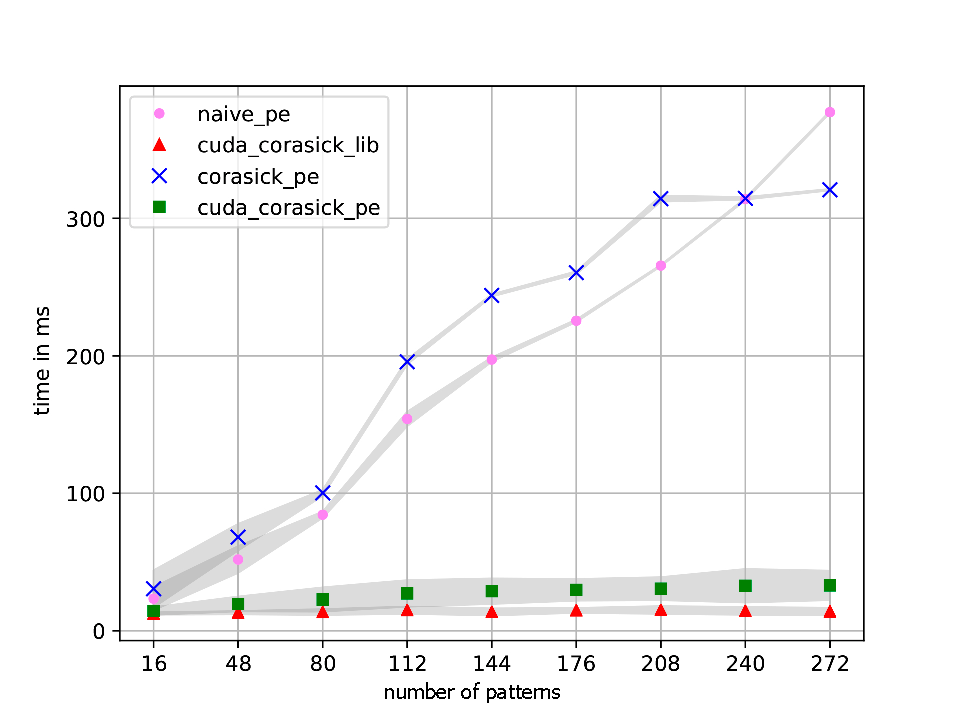
\includegraphics[width=\linewidth]{figures/PredDefendNaiveSearchorasick(eng).pdf}
    \caption{Aho-Corasick matching}
    \label{fig:my_corasick}
\end{figure}

Static binding is a traversal of statically known possible values of a dynamic 
parameter in a bunch of condition statements. In this case, such an approach 
induces more thread divergence, e.g. 6 times if compared to \emph{cuda\_corasick\_lib}, 
which drastically decreases the performance of a GPU application. 
The interpreter approach has better divergence behavior but still diverges 
twice as much as \emph{cuda\_corasick\_lib}. So, given that global memory access 
latency even on L1 cache hit is more than the one for embedded data, 
the static binding approach that could work well on a CPU has a poor 
performance when a GPU is used, and even if interpretative implementation is 
near, such an embedding also does not provide any performance benefit.

\subsection{Convolutional filtering}

\begin{figure}[h!]
    \centering
    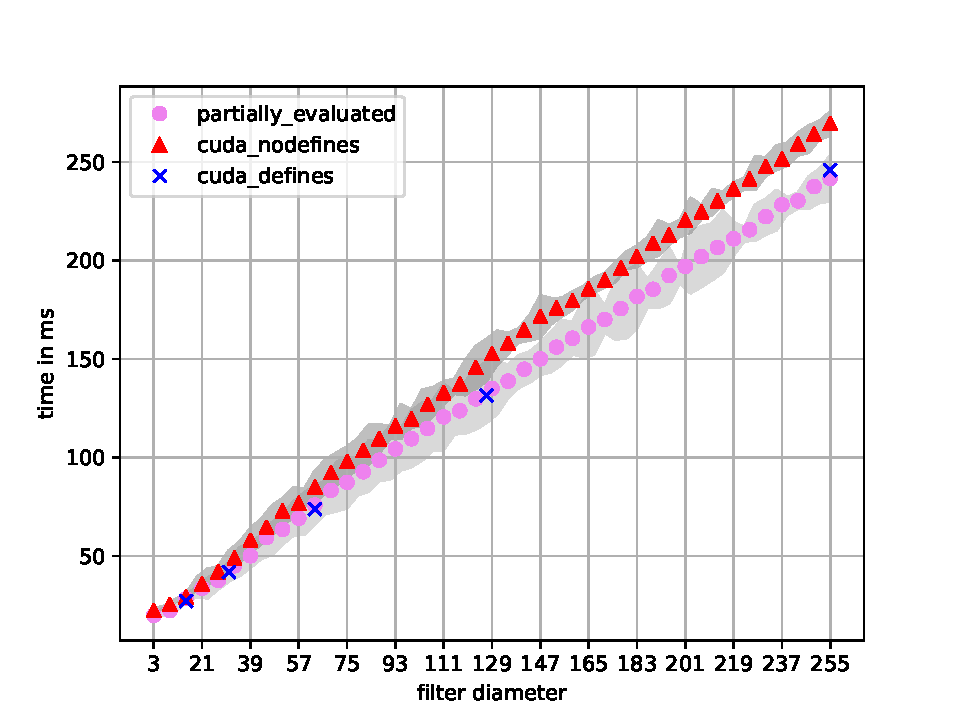
\includegraphics[width=\linewidth]{figures/separable_convolution_diploma.pdf}
    \caption{Separable convolution}
    \label{fig:convolution}
\end{figure}

Convolutional filtering is a matrix dot product frequently used in image processing~\cite{chetlur2014cudnn}. Basically, there are a huge subject matrix and a small filter matrix, and each submatrix of the subject matrix is dot producted with the filter matrix.
Since the filter is small and is static, the convolution operation could be partially evaluated with respect to the filter.
A partial evaluation for a 2-D separable\footnote{1-D filter could be applied first to rows and then to columns.} convolutional filtering has been performed in~\cite{OnlinePe}, targeting different hardware, however, the described filter is a rewritten modification of the reference filter, thus the obtained speed-up is not achieved by means of partial evaluator solely, and is used to demonstrate the facilities of the Impala language.

\subsubsection{Separable convolution}

A separable convolutional filter has been implemented in CUDA and 
Impala~\cite{CudaConv}. It operates on a 2-D array in global memory with 
threads organized in $32 x 16$ blocks, where each thread convolves 8 elements. 
Shared memory is utilized to store the big area for convolution with a block 
and the required borders. Since the filter is read-only and accessed equally 
by all the threads, it is stored in constant memory. Elements that fall away 
the borders of the 2-D subject array are assigned zeroes. 
There are two device kernels to perform a convolution: one convolves the rows 
and the other convolves the columns with the shared memory padded enough to 
not cause bank conflicts when accessing column elements.

\begin{listing}
    
\begin{pyglist}[language=C,label=code:conv,caption=Convolution partial evaluation]
//cuda_defines
LDS.U R16, [R2 + 0x38] //load from shared
FFMA R17, R10, c[0x3][0x1dc] R17 //float multiply add

//partially_evaluated
LDS.U R16, [R2 + 0x38] //load from shared
FFMA R17, R10, 42 R17 //float multiply add

\end{pyglist}
\end{listing}

The convolution itself is a dot product of two vectors of filter size. 
Since the size is known, this cycle could be unrolled with the filter being 
embedded. %In~\cite{OnlinePe} the partial evaluator generated different convolve functions for regions of the 2-D array that are near the borders (assigned with zeroes), and ones that are not, reducing the number of conditional statements. However, this is not portable on a GPU, since which thread block would operate on a borders area is a device kernel runtime information and thus is fully dynamic and could not be exploited. In
Such an unroll could be also performed by means of C++ templates or macros, by creating a dedicated device kernel for a specific filter size and dynamically dispatching the appropriate kernel for input data. The results of the benchmark are depicted in figure~\ref{fig:convolution}. The subject 2-D array is 1GB randomly generated, the filters are randomly generated for each diameter. The average has been taken for each filter size from 30 runs. The gray area is the standard deviation. \emph{Cuda\_nodefines} is the implementation with the dot product not unrolled, \emph{cuda\_defines} leverages macros to unroll the product, \emph{partially\_evaluated} leverages partial evaluation. Unrolled versions are at the bottom since they reduce the loop overhead. Unrolled version perform equally due to the code generated by the compiler as in listing~\ref{code:conv} which has been shown to be executed in the same number of cycles in~\ref{data_embedding}.
In~\cite{OnlinePe} the partial evaluator generated different convolve functions for regions of the 2-D array that are near the borders (assigned with zeroes), and ones that are not, reducing the number of conditional statements. However, this is not portable on a GPU, since which thread block would operate on a borders area is a device kernel runtime information and thus is fully dynamic and could not be exploited.


%The runtime compilation overhead could be estimated 
% Unlike possible fully dynamic thread divergence, induced by partial evaluation, i.e. divergence could differ in different runs depending on the data, compiler is static. Thus, in this case the possible performance could be as well statically estimated prior to running the kernel


\section{Заключение}

В данной работе описан подход к композициональному символьному исполнению без раскрутки. Была предложена концепция композициональной памяти с символьной адресацией. Был доказан некоторый набор свойств КСП, дающий основание для подхода в стиле систем переписывания, где символьные кучи могут сами выступать как символы. Это даёт возможность автоматически порождать уравнения на состояния, решения которых в точности отражают поведения функций, работающих с динамической памятью. Было показано как свести задачу решения уравнений на состояния к задаче проверки безопасности чистых функций второго порядка.

Данная работа нацелена на теоретические основания композиционального анализа динамической памяти. Мы оставляем апробацию этого подхода на будущее. Другим направлением будущих исследований может быть расширение нашего формализма на композициональный анализ параллельных программ.

%\begin{thebibliography}{99}
\begin{thebibliography}{10}
\def\selectlanguageifdefined#1{
\expandafter\ifx\csname date#1\endcsname\relax
\else\selectlanguage{#1}\fi}
\providecommand*{\href}[2]{{\small #2}}
\providecommand*{\url}[1]{{\small #1}}
\providecommand*{\BibUrl}[1]{\url{#1}}
\providecommand{\BibAnnote}[1]{}
\providecommand*{\BibEmph}[1]{#1}
\ProvideTextCommandDefault{\cyrdash}{\iflanguage{russian}{\hbox
  to.8em{--\hss--}}{\textemdash}}
\providecommand*{\BibDash}{\ifdim\lastskip>0pt\unskip\nobreak\hskip.2em plus
  0.1em\fi
\cyrdash\hskip.2em plus 0.1em\ignorespaces}
\renewcommand{\newblock}{\ignorespaces}

\bibitem{graph-propery-model}
\selectlanguageifdefined{english}
\BibEmph{Angles~Renzo}. The Property Graph Database Model~// AMW. \BibDash
\newblock 2018.

\bibitem{Azimov:2018:CPQ:3210259.3210264}
\selectlanguageifdefined{english}
\BibEmph{Azimov~Rustam, Grigorev~Semyon}.
  \href{http://dx.doi.org/10.1145/3210259.3210264}{Context-Free Path Querying
  by Matrix Multiplication}~// Proceedings of the 1st ACM SIGMOD Joint
  International Workshop on Graph Data Management Experiences \& Systems
  (GRADES) and Network Data Analytics (NDA). \BibDash
\newblock GRADES-NDA ’18. \BibDash
\newblock New York, NY, USA~: Association for Computing Machinery, 2018.
  \BibDash
\newblock Access mode: \BibUrl{https://doi.org/10.1145/3210259.3210264}
  (online; accessed: 29.05.2020).

\bibitem{FLCpathProblem}
\selectlanguageifdefined{english}
\BibEmph{Barrett~Chris, Jacob~Riko, Marathe~Madhav}.
  Formal-Language-Constrained Path Problems~//
  \href{http://dx.doi.org/10.1137/S0097539798337716}{\BibEmph{SIAM J. Comput.}}
  \BibDash
\newblock 2000. \BibDash May. \BibDash
\newblock Vol.~30, no.~3. \BibDash
\newblock P.~809–837. \BibDash
\newblock Access mode: \BibUrl{https://doi.org/10.1137/S0097539798337716}
  (online; accessed: 29.05.2020).

\bibitem{cfpq-data}
\selectlanguageifdefined{english}
CFPQ\_Data. Graphs and grammars for experimental analysis of context-free path
  querying algorithms. \BibDash
\newblock Access mode:
  \BibUrl{https://github.com/JetBrains-Research/CFPQ\_Data} (online; accessed:
  29.05.2020).

\bibitem{zhlang-2016}
\selectlanguageifdefined{english}
Context-free path queries on RDF graphs~/ X.~Zhang, Z.~Feng, X.~Wang et~al.~//
  International Semantic Web Conference~/ Springer. \BibDash
\newblock 2016. \BibDash
\newblock P.~632--648.

\bibitem{cypher-language}
\selectlanguageifdefined{english}
\href{http://dx.doi.org/10.1145/3183713.3190657}{Cypher: An Evolving Query
  Language for Property Graphs}~/ Nadime~Francis, Andrés~Taylor,
  Alastair~Green et~al. \BibDash
\newblock 2018. \BibDash 05. \BibDash
\newblock P.~1433--1445.

\bibitem{cypher-specification}
\selectlanguageifdefined{english}
Cypher extention. CIP2017-02-06 Path Patterns. \BibDash
\newblock Access mode:
  \BibUrl{https://github.com/thobe/openCypher/blob/rpq/cip/1.accepted/CIP2017-02-06-Path-Patterns.adoc}
  (online; accessed: 29.05.2020).

\bibitem{docker}
\selectlanguageifdefined{english}
Docker containter with RedisGraph fork. Context-free path queries support.
  \BibDash
\newblock Access mode: \BibUrl{https://hub.docker.com/r/simpletondl/redisgraph}
  (online; accessed: 29.05.2020).

\bibitem{azimov-evalution}
\selectlanguageifdefined{english}
\href{http://dx.doi.org/10.1145/3327964.3328503}{Evaluation of the Context-Free
  Path Querying Algorithm Based on Matrix Multiplication}~/ Nikita~Mishin,
  Iaroslav~Sokolov, Egor~Spirin et~al.~// Proceedings of the 2nd Joint
  International Workshop on Graph Data Management Experiences \& Systems
  (GRADES) and Network Data Analytics (NDA). \BibDash
\newblock GRADES-NDA’19. \BibDash
\newblock New York, NY, USA~: Association for Computing Machinery, 2019.
  \BibDash
\newblock Access mode: \BibUrl{https://doi.org/10.1145/3327964.3328503}.

\bibitem{Kuijpers:2019:ESC:3335783.3335791}
\selectlanguageifdefined{english}
\href{http://dx.doi.org/10.1145/3335783.3335791}{An Experimental Study of
  Context-Free Path Query Evaluation Methods}~/ Jochem~Kuijpers,
  George~Fletcher, Nikolay~Yakovets, Tobias~Lindaaker~// Proceedings of the
  31st International Conference on Scientific and Statistical Database
  Management. \BibDash
\newblock SSDBM '19. \BibDash
\newblock New York, NY, USA~: ACM, 2019. \BibDash
\newblock P.~121--132. \BibDash
\newblock Access mode: \BibUrl{http://doi.acm.org/10.1145/3335783.3335791}
  (online; accessed: 29.05.2020).

\bibitem{hellings-2015}
\selectlanguageifdefined{english}
\BibEmph{Hellings~Jelle}. Querying for Paths in Graphs using Context-Free Path
  Queries~// \BibEmph{arXiv preprint arXiv:1502.02242}. \BibDash
\newblock 2015.

\bibitem{graph-blas}
\selectlanguageifdefined{english}
\BibEmph{Jeremy~Kepner}. GraphBLAS Mathematics - Provisional Release 1.0.
  \BibDash
\newblock 2017. \BibDash
\newblock Access mode:
  \BibUrl{http://www.mit.edu/~kepner/GraphBLAS/GraphBLAS-Math-release.pdf}
  (online; accessed: 29.05.2020).

\bibitem{datascince-lifecycle}
\selectlanguageifdefined{english}
\BibEmph{Miao~Hui, Deshpande~Amol}. Understanding Data Science Lifecycle
  Provenance via Graph Segmentation and Summarization~// \BibEmph{2019 IEEE
  35th International Conference on Data Engineering (ICDE)}. \BibDash
\newblock 2019. \BibDash
\newblock P.~1710--1713.

\bibitem{neo4j}
\selectlanguageifdefined{english}
Neo4j. \BibDash
\newblock Access mode: \BibUrl{https://neo4j.com} (online; accessed:
  29.05.2020).

\bibitem{parser-combinators}
\selectlanguageifdefined{english}
\href{http://dx.doi.org/10.1145/3241653.3241655}{Parser Combinators for
  Context-Free Path Querying}~/ Ekaterina~Verbitskaia, Ilya~Kirillov,
  Ilya~Nozkin, Semyon~Grigorev~// Proceedings of the 9th ACM SIGPLAN
  International Symposium on Scala. \BibDash
\newblock Scala 2018. \BibDash
\newblock New York, NY, USA~: Association for Computing Machinery, 2018.
  \BibDash
\newblock P.~13–--23. \BibDash
\newblock Access mode: \BibUrl{https://doi.org/10.1145/3241653.3241655}
  (online; accessed: 29.05.2020).

\bibitem{geospices}
\selectlanguageifdefined{english}
\BibEmph{Peter~DeVries}. The GeoSpecies Knowledge Base ontology. \BibDash
\newblock 2009. \BibDash
\newblock Access mode: \BibUrl{http://rdf.geospecies.org/geospecies.rdf.gz}
  (online; accessed: 29.05.2020).

\bibitem{redis}
\selectlanguageifdefined{english}
Redis. Open source (BSD licensed), in-memory data structure store. \BibDash
\newblock Access mode: \BibUrl{https://redis.io} (online; accessed:
  29.05.2020).

\bibitem{redis-graph}
\selectlanguageifdefined{english}
RedisGraph. Graph database module for Redis. \BibDash
\newblock Access mode: \BibUrl{https://oss.redislabs.com/redisgraph} (online;
  accessed: 29.05.2020).

\bibitem{github}
\selectlanguageifdefined{english}
RedisGraph fork. Context-free path queries support. \BibDash
\newblock Access mode:
  \BibUrl{https://github.com/YaccConstructor/RedisGraph/tree/path_patterns}
  (online; accessed: 29.05.2020).

\bibitem{santos-2018}
\selectlanguageifdefined{english}
\BibEmph{Santos~Fred~C., Costa~Umberto~S., Musicante~Martin~A.} A Bottom-Up
  Algorithm for Answering Context-Free Path Queries in Graph Databases~// Web
  Engineering~/ Ed.\ by\ Tommi~Mikkonen, Ralf~Klamma, Juan~Hern{\'a}ndez.
  \BibDash
\newblock Cham~: Springer International Publishing, 2018. \BibDash
\newblock P.~225--233.

\bibitem{bio-application}
\selectlanguageifdefined{English}
\BibEmph{Sevon~Petteri, Eronen~Lauri}. Subgraph queries by context-free
  grammars~// \BibEmph{Journal of Integrative Bioinformatics : JIB}. \BibDash
\newblock 2008. \BibDash
\newblock Vol.~5, no. 100, 16 s.

\bibitem{suite-sparse}
\selectlanguageifdefined{english}
SuiteSparse. A suite of sparse matrix software. \BibDash
\newblock Access mode: \BibUrl{http://faculty.cse.tamu.edu/davis} (online;
  accessed: 29.05.2020).

\end{thebibliography}

  
%\end{thebibliography}
  
